% $Id: template.tex 11 2007-04-03 22:25:53Z jpeltier $

%\documentclass{vgtc}                          % final (conference style)
\documentclass[review]{vgtc}                 % review
%\documentclass[widereview]{vgtc}             % wide-spaced review
%\documentclass[preprint]{vgtc}               % preprint
%\documentclass[electronic]{vgtc}             % electronic version

%% Uncomment one of the lines above depending on where your paper is
%% in the conference process. ``review'' and ``widereview'' are for review
%% submission, ``preprint'' is for pre-publication, and the final version
%% doesn't use a specific qualifier. Further, ``electronic'' includes
%% hyperreferences for more convenient online viewing.

%% Please use one of the ``review'' options in combination with the
%% assigned online id (see below) ONLY if your paper uses a double blind
%% review process. Some conferences, like IEEE Vis and InfoVis, have NOT
%% in the past.

%% Figures should be in CMYK or Grey scale format, otherwise, colour 
%% shifting may occur during the printing process.

%% These few lines make a distinction between latex and pdflatex calls and they
%% bring in essential packages for graphics and font handling.
%% Note that due to the \DeclareGraphicsExtensions{} call it is no longer necessary
%% to provide the the path and extension of a graphics file:
%% \includegraphics{diamondrule} is completely sufficient.
%%
\ifpdf%                                % if we use pdflatex
  \pdfoutput=1\relax                   % create PDFs from pdfLaTeX
  \pdfcompresslevel=9                  % PDF Compression
  \pdfoptionpdfminorversion=7          % create PDF 1.7
  \ExecuteOptions{pdftex}
  \usepackage{graphicx}                % allow us to embed graphics files
  \DeclareGraphicsExtensions{.pdf,.png,.jpg,.jpeg} % for pdflatex we expect .pdf, .png, or .jpg files
\else%                                 % else we use pure latex
  \ExecuteOptions{dvips}
  \usepackage{graphicx}                % allow us to embed graphics files
  \DeclareGraphicsExtensions{.eps}     % for pure latex we expect eps files
\fi%

%% it is recomended to use ``\autoref{sec:bla}'' instead of ``Fig.~\ref{sec:bla}''
\graphicspath{{figures/}{pictures/}{images/}{./}} % where to search for the images

\usepackage{microtype}                 % use micro-typography (slightly more compact, better to read)
\PassOptionsToPackage{warn}{textcomp}  % to address font issues with \textrightarrow
\usepackage{textcomp}                  % use better special symbols
\usepackage{mathptmx}                  % use matching math font
\usepackage{times}                     % we use Times as the main font
\renewcommand*\ttdefault{txtt}         % a nicer typewriter font
\usepackage{cite}                      % needed to automatically sort the references
\usepackage{tabu}                      % only used for the table example
\usepackage{booktabs}                  % only used for the table example
%% We encourage the use of mathptmx for consistent usage of times font
%% throughout the proceedings. However, if you encounter conflicts
%% with other math-related packages, you may want to disable it.
\usepackage[T1]{fontenc}
\usepackage{lmodern}

\usepackage{booktabs} % For formal tables
\usepackage{array}
\newcolumntype{C}[1]{>{\centering\let\newline\\\arraybackslash\hspace{0pt}}m{#1}}
\usepackage{subcaption}
\usepackage{url}
\usepackage{acronym}
\usepackage{color}
\usepackage{amsmath}
%% If you are submitting a paper to a conference for review with a double
%% blind reviewing process, please replace the value ``0'' below with your
%% OnlineID. Otherwise, you may safely leave it at ``0''.
\onlineid{1183}

%% declare the category of your paper, only shown in review mode
\vgtccategory{S\&T Papers}

%% allow for this line if you want the electronic option to work properly
%\vgtcinsertpkg

%% In preprint mode you may define your own headline.
%\preprinttext{To appear in an IEEE VGTC sponsored conference.}

%% Paper title.
\acrodef{dtw}[DTW]{Dynamic Time Warping}
\acrodef{lstm}[LSTM]{Long Short-Term Memory}
\acrodef{doctic}[DOCTIC]{Dual-Check Till Consensus}
\acrodef{har}[HAR]{Human Activity Recognition}
\acrodef{hmm}[HMM]{Hidden Markov Model}


\title{Accurate and Fast Classification of Foot Gestures for Virtual Locomotion}

%% This is how authors are specified in the conference style

%% Author and Affiliation (single author).
%%\author{Roy G. Biv\thanks{e-mail: roy.g.biv@aol.com}}
%%\affiliation{\scriptsize Allied Widgets Research}

%% Author and Affiliation (multiple authors with single affiliations).
%%\author{Roy G. Biv\thanks{e-mail: roy.g.biv@aol.com} %
%%\and Ed Grimley\thanks{e-mail:ed.grimley@aol.com} %
%%\and Martha Stewart\thanks{e-mail:martha.stewart@marthastewart.com}}
%%\affiliation{\scriptsize Martha Stewart Enterprises \\ Microsoft Research}

%% Author and Affiliation (multiple authors with multiple affiliations)
\author{Roy G. Biv\thanks{e-mail: roy.g.biv@aol.com}\\ %
        \scriptsize Starbucks Research %
\and Ed Grimley\thanks{e-mail: ed.grimley@aol.com}\\ %
     \scriptsize Grimley Widgets, Inc. %
\and Martha Stewart\thanks{e-mail: martha.stewart@marthastewart.com}\\ %
     \parbox{1.4in}{\scriptsize \centering Martha Stewart Enterprises \\ Microsoft Research}}

%% A teaser figure can be included as follows, but is not recommended since
%% the space is now taken up by a full width abstract.
%\teaser{
%  \includegraphics[width=1.5in]{sample.eps}
%  \caption{Lookit! Lookit!}
%}

%% Abstract section.
\abstract{
This work explores the use of foot gestures for locomotion in virtual environments. 
Foot gestures are represented as the distribution of plantar pressure and detected by three sparsely-located sensors on each insole. 
% The trained classifier can successfully recognize the performer's behaviour based on the captured signals of pressure information.
The \acl{lstm} model is chosen as the classifier to recognize the performer's foot gesture based on the captured signals of pressure information.
The trained classifier directly takes the noisy and sparse input of sensor data, and handles seven categories of foot gestures (stand, walk forward/backward, run, jump, slide left and right) without manual definition of signal features for classifying these gestures.
This classifier is capable of recognizing the foot gestures, even with the existence of large sensor-specific, inter-person and intra-person variations.
Results show that an accuracy of $\sim$80\% can be achieved across different users with different shoe sizes and $\sim$85\% for users with the same shoe size.
A novel method, \acl{doctic}, is proposed to reduce the latency of gesture recognition from 2 seconds to 0.5 seconds and increase the accuracy to over 97\%.
This method offers a promising solution to achieve lower latency and higher accuracy at a minor cost of computation workload.
The characteristics of high accuracy and fast classification of our method could lead to wider applications of using foot patterns for human-computer interaction.
} % end of abstract

%% ACM Computing Classification System (CCS). 
%% See <http://www.acm.org/about/class> for details.
%% We recommend the 2012 system <http://www.acm.org/about/class/class/2012>
%% For the 2012 system use the ``\CCScatTwelve'' which command takes four arguments.
%% The 1998 system <http://www.acm.org/about/class/class/2012> is still possible
%% For the 1998 system use the ``\CCScat'' which command takes four arguments.
%% In both cases the last two arguments (1998) or last three (2012) can be empty.

\CCScatlist{
  \CCScatTwelve{Human-centered computing}{Human computer interaction (HCI)}{Interaction techniques}{Gestural input};
  \CCScatTwelve{Human-centered computing}{Human computer interaction (HCI)}{Interactive systems and tools}{User interface programming}
}

%\CCScatlist{
  %\CCScat{H.5.2}{User Interfaces}{User Interfaces}{Graphical user interfaces (GUI)}{};
  %\CCScat{H.5.m}{Information Interfaces and Presentation}{Miscellaneous}{}{}
%}

%% Copyright space is enabled by default as required by guidelines.
%% It is disabled by the 'review' option or via the following command:
% \nocopyrightspace

%%%%%%%%%%%%%%%%%%%%%%%%%%%%%%%%%%%%%%%%%%%%%%%%%%%%%%%%%%%%%%%%
%%%%%%%%%%%%%%%%%%%%%% START OF THE PAPER %%%%%%%%%%%%%%%%%%%%%%
%%%%%%%%%%%%%%%%%%%%%%%%%%%%%%%%%%%%%%%%%%%%%%%%%%%%%%%%%%%%%%%%%

\begin{document}
\newcommand{\shihuinote}[1]{\textcolor{red}{#1}}
%% The ``\maketitle'' command must be the first command after the
%% ``\begin{document}'' command. It prepares and prints the title block.

%% the only exception to this rule is the \firstsection command
%\firstsection{Introduction}

\maketitle

%% \section{Introduction} %for journal use above \firstsection{..} instead
%This template is for papers of VGTC-sponsored conferences which are \emph{\textbf{not}} published in a special issue of TVCG.

\section{Introduction}
\label{sec:introduction}
The rapid development of consumer-level devices for Virtual Reality (VR), such as Oculus and HTC Vive, leads to an increasing popularity among the public.
The immersion in virtual environments (VEs) offers unique experiences to users and shows its potential in the fields of education, broadcasting, entertainment etc.
The capability of freely navigating in a large VE is a critical function in interactive VR applications.
A recent work \cite{nilsson2018natural} reviewed the efforts to perform natural walking in VEs.
Compared with walking-in-place and joystick-based locomotion, real walking serves as a better mode of locomotion in terms of simplicity, straightforwardness, naturalness \cite{usoh1999walking,dong2017smooth,nilsson2018natural}.

However, it is a challenging task to map the locomotion in real world (RW) to that in the VE.
The first challenge is to capture the locomotion pattern in real world.
Standard motion capture systems, such as Vicon, are expensive and require additional efforts in setting up the external devices (specialized cameras and tracking suits).
Although alternative solutions, such as Kinect, Oculus Quest and Vive Focus, allow fast setup and accurate tracking, users are still physically constrained in a limited space and may not be able to use such devices in challenging scenarios such as outdoor environments.
The second challenge is to define the mapping from the captured posture in the RW to the \emph{referent} action \cite{felberbaum2018better} in the VE, in particularly in the case of walking-in-place where there are no direct mapping rules.
Researchers have proposed various walking-in-place methods (GUD-WIP \cite{wendt2010gud}, LLCM-WIP \cite{feasel2008llcm} and SAS-WIP \cite{bruno2013new}), or hybrid methods (Legomotion \cite{bhandari2017legomotion}), to allow users to explore a large VE by walking in a relatively small RW.
However, existing methods generally require manual-tuning of parameters to identify different motion categories and are limited to most-common gestures (walking-stopping).
Therefore, it is still important to develop alternative methods to allow intuitive exploration in the VE. 

Inspired by the fact that we wear shoes to facilitate long-distance locomotion, this work uses sensors in the insoles to detect the plantar pressure and capture the locomotion patterns in the RW (Figure~\ref{fig:teaser}).
Although foot gestures serve as a promising solution for interaction
(see \cite{velloso2015feet} for a comprehensive review in this domain and some recent works \cite{fukahori2015exploring,tajadura2015light,matthies2017capsoles}), it is significantly difficult to interpret the signal of pressure distributions given a large group of users and a wide range of locomotion patterns. 
The reasons are threefold. 
First, there exist \textbf{sensor-specific} variations in the manufacture process, which means two sensors may return different pressure values even though they are pressed with the same force. 
Second, we observe large \textbf{inter-person} and \textbf{intra-person} variations, which means such signals of the same pattern may vary significantly for different persons, or even for the same person when making different attempts. 
Third, 
%the number of pressure sensors can critically determine the classification performance, but
using excessive number of sensors may introduce redundant information and increase the manufacture and computing cost, while using a minimal number of sensors may require longer sequences to accurately identify the locomotion pattern.
Therefore, developing a stable and fast classification algorithm to handle noisy and sparse data is a non-trivial task.

\begin{figure}
	\centering
	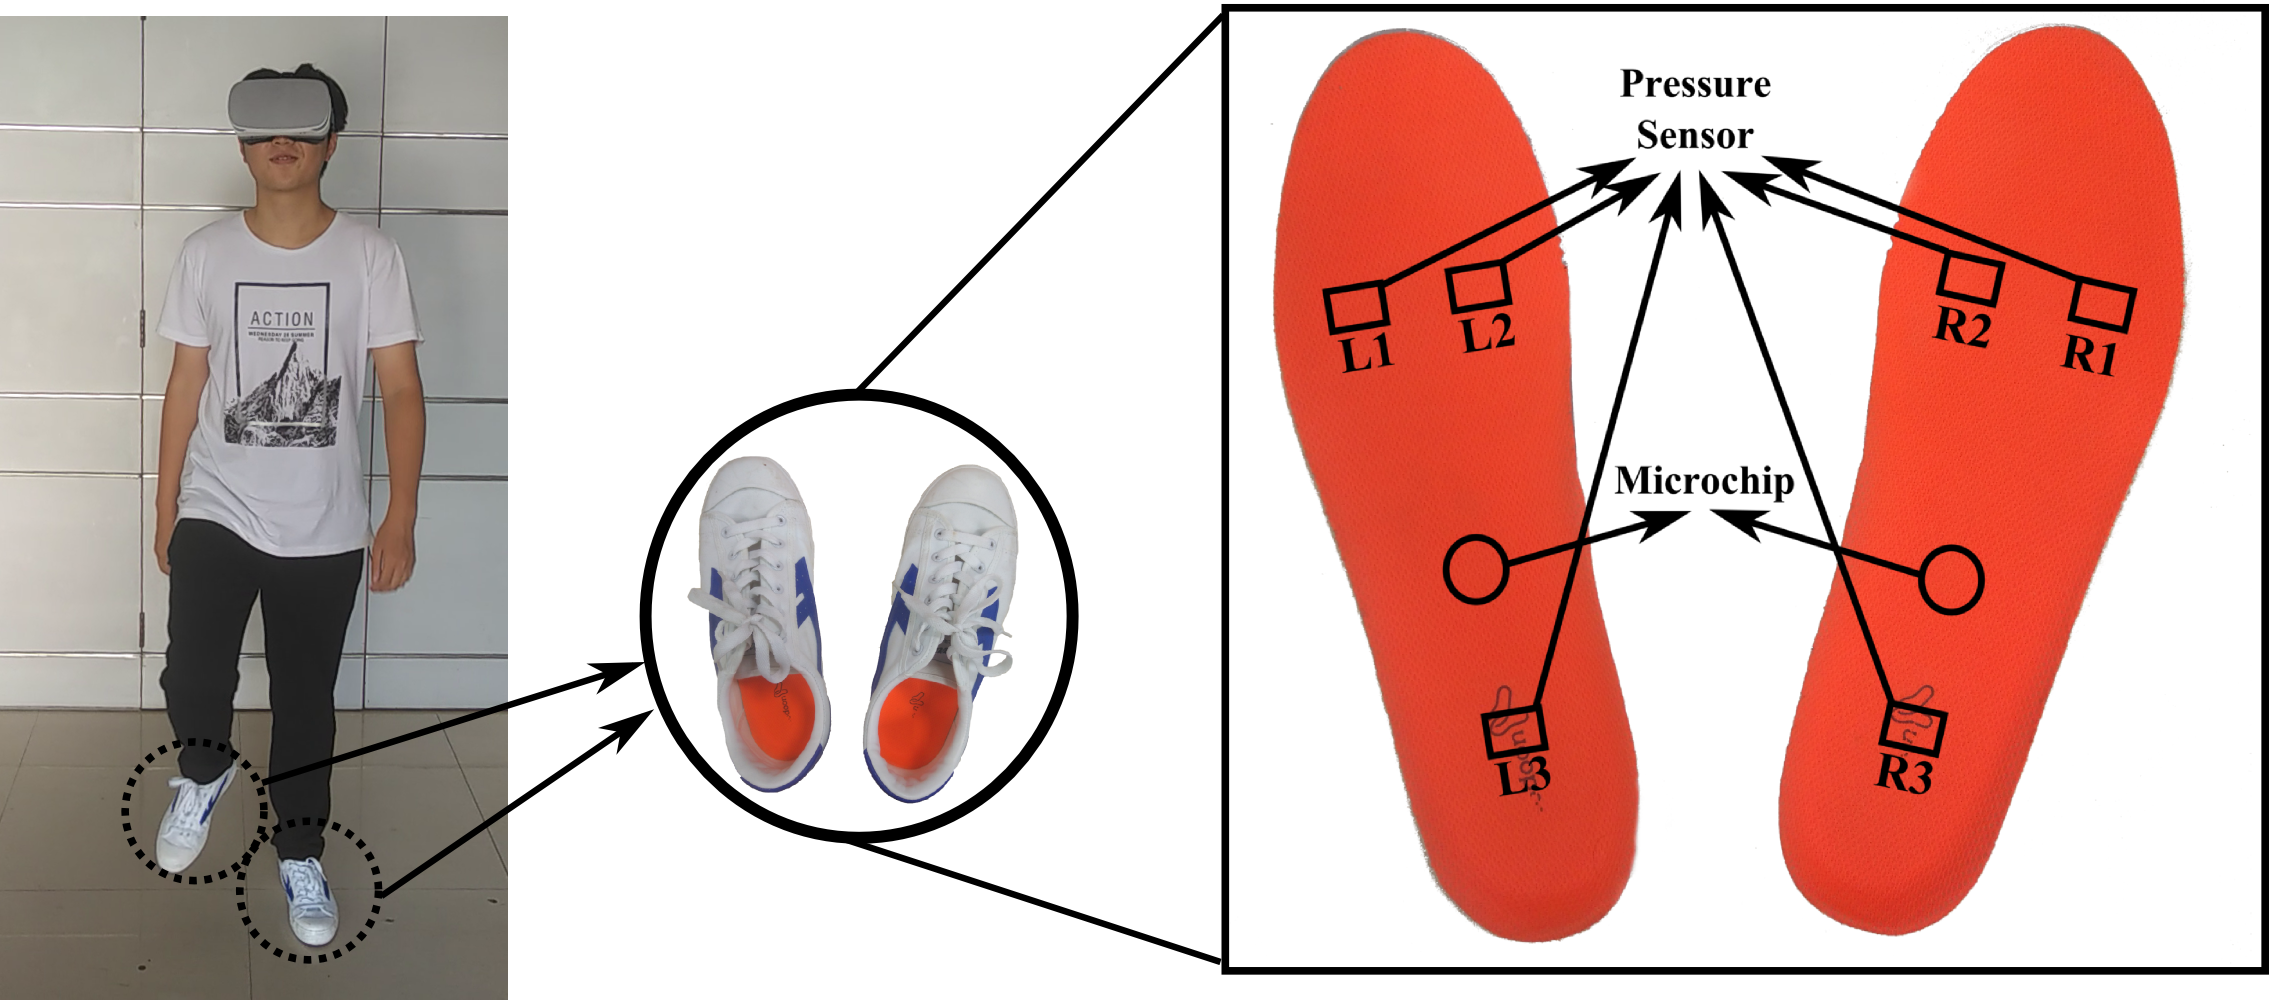
\includegraphics[width=\linewidth]{figs/teaser.png}
	\caption{(left) user performing the walking with the device. (middle) shoes with smart insoles. (right) smart insoles with the illustration of the location of pressure sensors and microchip.}
	\label{fig:teaser}
\end{figure}

% There are two goals in this study: 
% 1) explore a set of natural foot patterns for interaction with VR applications, and evaluate the user experience in using these foot patterns to navigate in a large-scale VE; 
The goal of this study is to develop novel techniques with sparse distribution of plantar pressure and achieve accurate and fast classification of foot gestures for virtual locomotion.
We use consumer-level hardware (for the retail price of 30USD), with three pressure sensors sparsely embedded in each insole.
This classifier should be robust against noises caused by sensor and individual variations, and capable of identifying the accurate foot patterns within a short time frame.	
In addition to well-investigated walking/stopping patterns, we also aim to explore a wider range of other gestures for intuitive interaction in VE.
To this end, we made the following contributions:
\begin{itemize}
	\item We develop a pattern classifier, based on the \acf{lstm} network, which is generalized across different sensors and individuals. This classifier allows users to stand, walk forward/backward, run, jump, slide left and right, without manual definition of signal features. This is, to the best of authors' knowledge, the state-of-the-art numbers (N=7) of foot patterns, considering the large sensor-specific, inter-person and intra-person variations.
	\item We propose a novel method, \acf{doctic}, to make fast and accurate decisions on gesture recognition.
	In comparison to the standard \acs{lstm} network, \acs{doctic} achieves lower latency and higher accuracy at a minor cost of computation workload.
	The time latency is reduced from 2 seconds of the standard \acs{lstm} to 0.5 seconds while the accuracy is improved from 85\% to 97.1\%.
	\item We demonstrate the potential of our interaction technique in two applications: real walking in an office environment and walking-in-place in an interactive game. These experiments prove that our method as a complete solution enables users to intuitively explore the VE with the selected foot gestures. 
	%This solution includes the off-the-shelf insoles with embedded sensors, a set of foot gestures based on existing literature and our proposed classifier for gesture recognition. 

\end{itemize}


\section{Related Work}
%Gait analysis is an important procedure used to evaluate human locomotion and is a promising way to facilitate medical diagnostics, physical rehabilitation as well as sport risk prevention. However, traditional gait analysis has to be performed in a specific gait lab and operated by a medical professional with exorbitant cost and significant inconvenience. The smart insole, a wearable system embedded with the pressure sensors, is capable of collecting sufficient plantar information and serves as an alternative solution for gait analysis.

\subsection{Techniques for Virtual Locomotion}
Virtual locomotion refers to the functionality of allowing users to navigate in 3D virtual environments, which critically affects user's sense of presence.
We here focus on existing techniques using body (in particular foot) movements to trigger virtual locomotion, and exclude the discussions on using conventional devices (such as joy-stick, mouse, keyboard or touch screen).
So far researchers have proposed the techniques of real walking \cite{usoh1999walking,sun2016mapping,dong2017smooth}, walking-in-place \cite{yan2004new, wendt2010gud, feasel2008llcm, bruno2013new}, or hybrid solutions of real walking and walking-in-place \cite{bhandari2017legomotion,arnskov2018threefold}.
Experiments reveal the subject preferences of virtual locomotion techniques, in the orders of real walking, walking-in-place, flying and using button-like controller \cite{slater1995taking, templeman1999virtual, usoh1999walking}.
Although real walking \cite{usoh1999walking} offers users with high fidelity of presence and immersion, it is limited by the space size of real world.
The technique of redirected walking \cite{sun2016mapping,dong2017smooth} introduces subtle adjustment to the virtual path by translation, rotation, and curvature gains without affecting the user perception.
These adjustments allow users to walk in a substantially larger virtual space in a relatively smaller physical world.

Walking-in-place enjoys its advantages in allowing users to navigate in a large virtual space within a physically-constrained real world.
Advanced omni-directional treadmill has been developed to allow users to walk in all directions, however the high price of this device indicates that it is currently limited to professional scenarios, rather than consumer-level applications.
So far, representative walking-in-place techniques include GUD-WIP \cite{wendt2010gud}, LLCM-WIP \cite{feasel2008llcm}, SAS-WIP \cite{bruno2013new}), or hybrid methods (Legomotion \cite{bhandari2017legomotion}).
%Researchers also studied the relationship between the real and perceived walking speed, and the effect of the display Field-of-View size on the perceived speed.
In addition to the use of foot, virtual locomotion has been achieved with non-critical body parts, including tapping \cite{nilsson2013tapping}, hip bending and leaning \cite{langbehn2015evaluation,guy2015lazynav,punpongsanon2017extended}, shaking-head \cite{terziman2010shake}, arm swing \cite{nilsson2013perceived}.
Researchers used other body-relevant devices, such as Wii balance board \cite{de2008using} or human-scale joystick \cite{marchal2011joyman}.
Researchers also explored the use of hip bending and leaning, for the purpose of ground navigation in scenarios of large display \cite{guy2015lazynav} and head-mounted display \cite{punpongsanon2017extended}.
We kindly refer our readers to recent surveys \cite{nilsson2016walking,nilsson2018natural} on details on natural walking in virtual reality.
The implementation of existing methods for walking-in-place involves manual efforts of tuning the threshold values for recognizing different actions, such as start and stop.
This process can be labour-intensive if the number of gestures increases.
Our work automatically identifies the signal features embedded in a large database and avoids the manual tuning of model parameters for the purpose of gesture classification. 




\subsection{Applications of Foot Interactions in Virtual Reality} 
Foot interactions in VR cover a wider range of channels, in addition to the aforementioned virtual locomotion.
Audio and haptics are two common interactions explored in existing studies \cite{nordahl2010preliminary,nordahl2011sound,papetti2010audio,nordahl2011multimodal,nordahl2012enhancing}.
Researchers developed shoes with pressure sensors, actuators, and markers and provided physically based audio-haptic feedback to users when they are virtually walking on different surfaces \cite{nordahl2012enhancing}.
This study reveals that although auditory and haptic feedback lead to a more realistic experience (reported by participants), this claim is not supported by experimental data and questionnaire.
A pair of haptic shoes, named RealWalk \cite{son2018realwalk}, adopted MR fluid (Magnetorheological fluid) actuators to simulate four different scenarios: grassland, snow, concrete floor and dry sand. 
MR fluid actuators adaptively adjust the viscosity of MR fluid by varying the magnetic field intensity based on the type of materials in virtual ground surfaces and the foot pressure distribution. 
Researchers also explored the use of foot gestures \cite{lv2014foot}, or in combination with hand \cite{lu2013hand}, as the interaction technique for mobile games. 
The information of foot pressure captured from a sensor pad is also used to interactively control avatars \cite{yin2003footsee}.
This system allows users to create interactive animations without the cost or inconveniences of a full body motion capture system.

Another application of foot patterns in the VR domain is an unobtrusive and immersive mobility training system for stroke rehabilitation called VRInsole \cite{oagaz2018vrinsole}. 
This system utilized the patients' motion information collected from the smart insole and thus provided the input for the VR application to perform corresponding exercise animations. 
Researchers \cite{lu2013hand} also designed an immersive football game on the platform of mobile phone and used hand/foot gestures to interact in this VE.
A proof of concept, named as ShoeSoleSense \cite{matthies2013shoesolesense}, was developed which enabled location independent hands-free interaction through the feet.
This device allows movement control, including moving straight, turning and jumping, in a virtual reality installation.
Researchers conducted user experiments to find out the best areas for measuring pressure.
Our work differentiates from existing works in that we focus on accurate and fast classification of foot patterns across different individuals, and apply such an interaction technique for exploring the 3D VEs.


\subsection{Hardware and Software for Foot Pattern Recognition} 
In order to capture foot patterns, popular solutions of sensor set-up include embedding the pressure sensors on the insole, attaching an accelerometer for measuring linear acceleration and a gyroscope for measuring orientation and angular velocity. 
% The number of pressure sensors in existing works varies from 8 \cite{manupibul2014design} to 1040 \cite{wu2015energy}.
Researchers embedded 48 pressure sensors into the insole to monitor the walking pattern and acquired the information including the walking speed, stride length and the cadence during the locomotion \cite{xu2012smart}. 
FootStriker \cite{daiber2017footstriker}, an EMS-based foot strike assistant, used force sensitive resistors (FSR) in the insole to detect the running style of users and Electrical Muscle Stimulation (EMS) as a real-time assistant to intuitively aid the runner in adapting a mid- or fore-foot stride pattern. 
Researchers also utilized other devices, such as Kinect, to track the foot gestures for Desktop 3D interaction \cite{simeone2014feet,velloso2015interactions}.
An in-shoe electronics system is developed to monitor temperature, pressure, and humidity for patients with diabetes and peripheral neuropathy \cite{morley2001shoe}.

Continuous collection and transmission of the pressure information require a substantial degree of power supply, which greatly limits the wide applications of the smart insole. 
The straightforward solution is reducing the sampling rate at the expense of data accuracy. 
A more recent research \cite{wu2015energy} increased the battery life from 2 to 10 hours with an energy-efficient adaptive sensing framework.
% to address this problem. 
Their solution is adaptively reducing the sampling density while preserving information fidelity based on the gait cycle analysis. 
%Through their efforts, the duration of the smart insole system with 52$\times$20 sensors has been increased from 2 hours to 10.47 hours.

As the technology of sensor manufacture gradually matures, researchers and entrepreneurs have made remarkable progress in offering commercial products of smart insoles  to the public.
The choices include Sennopro InsoleX \cite{wearable2016}, StepRite Insole \cite{roden2014development}, Brilliant Sole \cite{virtual} for various purposes of rehabilitation and training.
Instead of proposing a new system and duplicating the efforts of hardware design, our work uses an existing commercial product and focuses on developing a capable classifier with high accuracy and low latency.
Common algorithms in existing works of foot pattern recognition include peak detection and signal denoising. 
The peak detection method \cite{mladenov2009step,tumkur2012modeling,cho2017design} is widely used to detect the timing of foot strike and liftoff and calculate the time difference between two consecutive steps. 
Researchers compared the average pressure level between the left and right feet and evaluated the rate of the distortion in walking \cite{cho2017design}. 
The location, velocity and trajectory of Center-of-Pressure are computed as weighted formulas of the original pressure distributions \cite{lin2016smart}.
A major issue of the existing methods in recognizing foot gesture is the challenge to tackle the variations from different persons and sensors.
Our work uses the deep neural network to improve this capability of generalization.

%As the technology of smart insole gradually matures, researchers have made remarkable contributions in promoting the commercialization of this novel technology and making it available to the public. Some representative choices are Sennopro InsoleX \cite{wearable2016}, StepRite Insole \cite{roden2014development} and Brilliant Sole \cite{virtual}.
%Our work uses an existing commercial product, instead of proposing a new system.
%\subsection{Human Gesture Recognition using Wearable Sensors}
%A general-purpose framework for \acf{har} comprises stages for data acquisition, signal preprocessing and segmentation, feature extraction and selection, training, and classification \cite{bulling2014tutorial}.
%The challenges of \acs{har} include intra-class variability, inter-class similarity, which also significantly affect the recognition accuracy in our problem.
% The issue of intra-class variability is directly related to the observations of inter-person and intra-person variations  (as discussed in Section~\ref{sec:introduction}).
%The issues of inter-class variability and inter-class similarity 

%The increasing accessibility of wearable sensors leads to the fast development of HAR in recent years.
%The types of sensors include accelerometer, GPS, heart monitor, ECG, light sensor, thermometer, pressure sensor etc \cite{bulling2014tutorial}.
%Researchers proposed an algorithm to analyze readings from six on-body accelerometers to identify the soldier activity in the field \cite{minnen2007recognizing}.
%Given the wide popularity of the smart phone, using the readings from accelerometer and gyroscope on the phone is a convenient solution for the purpose of HAR \cite{anguita2012human,schneider2013real}. 
%Researchers utilized smart insoles to facilitate measurement of walking activities in a free-living nonrestrictive environment and improve lower limb motor function for stroke survivors \cite{davies2016personalized}.


%\subsection{Commercial Products of Smart Sole} 
%	As the technology of smart insole gradually matures, researchers have made remarkable contributions in promoting the commercialization of this novel technology and making it available to the public. Some representative choices are listed as follows:
%\begin{itemize}
%\item Sennopro InsoleX \cite{wearable2016}: It allows for measuring high-resolution foot pressure distribution and capturing gait data and thus has the capability of providing the players with a brand new immersive experience in virtual reality games. 
%\item StepRite Insole \cite{roden2014development}: Three main components are integrated into each of the two insoles: 4 force sensors, 2 accelerometers and a transmitter used to collect and transmit data to the data controller. They demonstrate two applications with this product: StepRite, which is applied for the purpose of rehabilitation exercises and RPM, which is developed to measure and monitor the athletes’ training performance.
%\item Brilliant Sole \cite{virtual}: This product is designed as the locomotion control solution for VR and video games. It can translate real movements of users (walking-in-place directionally, strafing, forward or reverse) into the manipulation over the game scene.
%\end{itemize}

\begin{figure*}
	\centering
	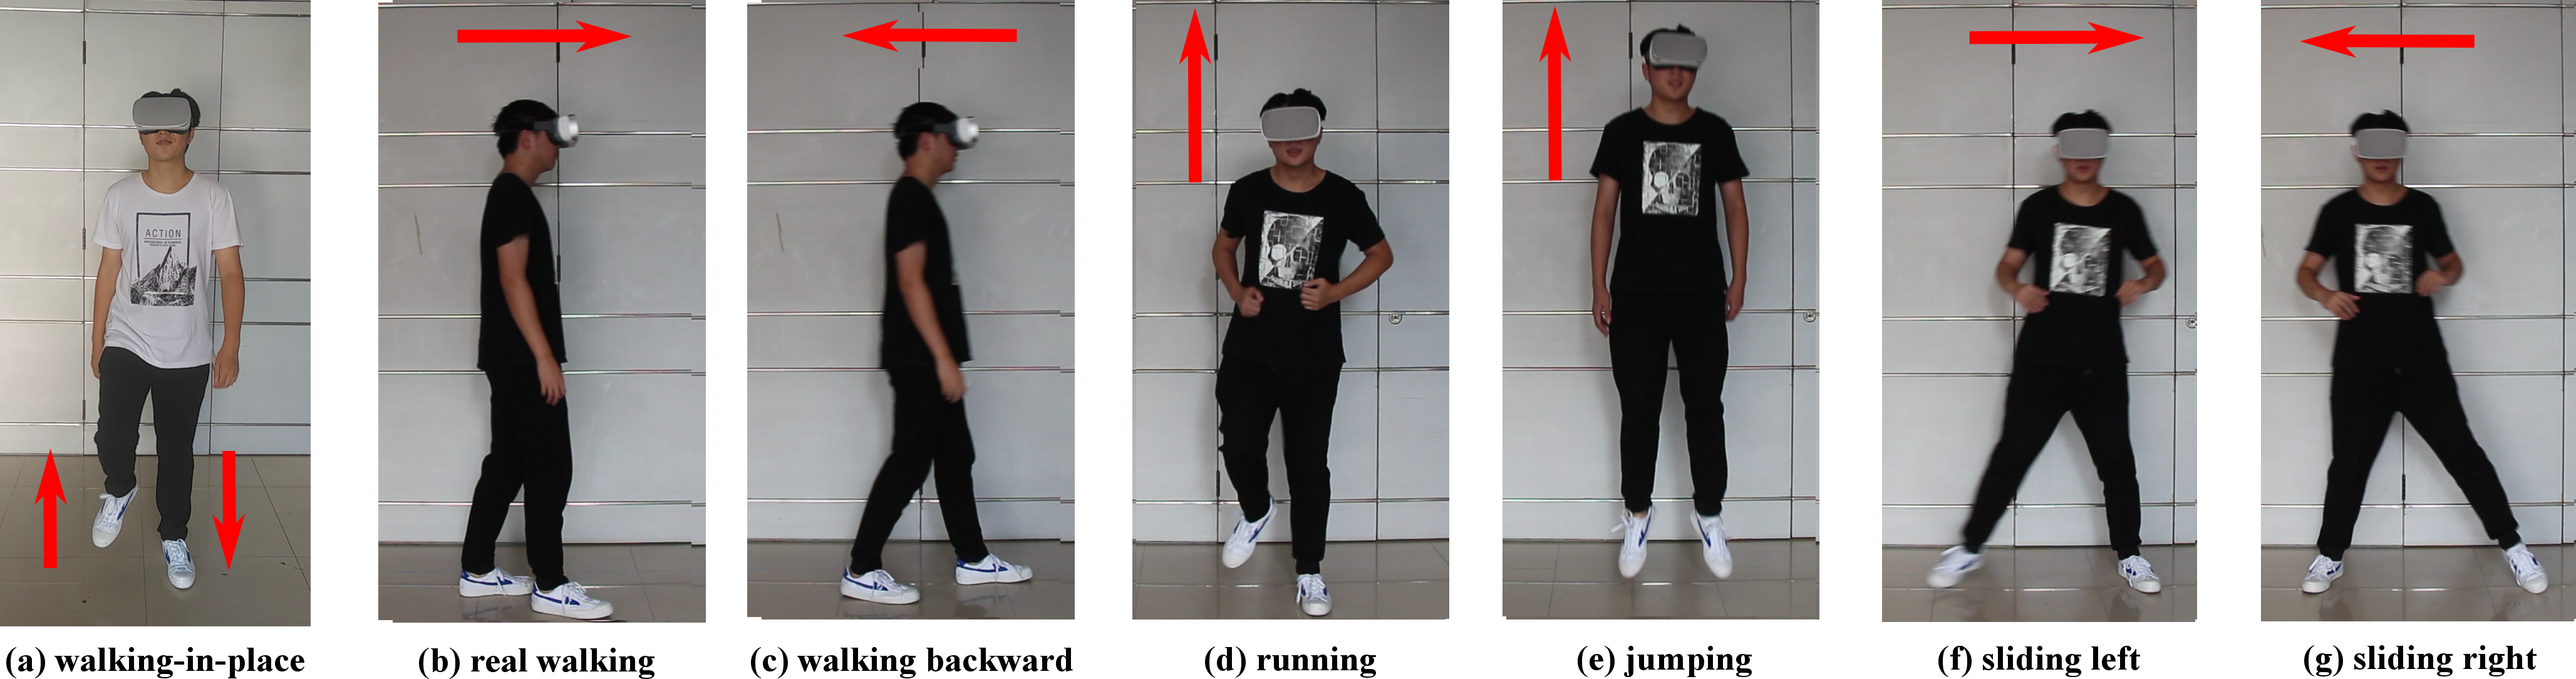
\includegraphics[width=\textwidth]{figs/gestures.png}
	\caption{Motion patterns to trigger the \emph{referents} of walking forward, backward, running, jumping, sliding left and right in VE.}
	\label{fig:gestures}
\end{figure*}


\section{Method Overview}
The goal of this work is to develop a method to accurately and fast classify foot gestures for virtual locomotion.
This section first explains the hardware and software implementation of our framework, followed by explanations on selected gestures in this work.
%The procedure of data collection and classifier training is detailed in Section.
%  collect the data from 32 participants in 3 different shoe sizes and complete the training of the pattern classifier based on the \acs{lstm} model.
Section~\ref{sec:training} presents a novel method, \acs{doctic}, which improve the standard \acs{lstm} model by reducing the time latency and increasing the classification accuracy.
The user study and its findings are presented in Section~\ref{sec:userstudy}.
We compared the performance of our work with state-of-the-art in Section~\ref{sec:discussions} and demonstrate two applications of our interaction technique in Section~\ref{sec:applications}.
Section~\ref{sec:conclusion} concludes this work and points out future directions.
%The trained classifier is integrated in three demonstrative applications to validate the selected patterns and relevant algorithms (Section~\ref{sec:validation}).
%Comparison experiments with existing methods, together with relevant discussions, are presented in Section~\ref{sec:result}.

\subsection{Hardware and Software Implementation}
We use the smart insole from Podoon Technology Ltd. \footnote{http://www.runmaf.com/} to complete this research. 
Their product is originally designed for athletes and enthusiasts of running, to record and improve their running gait using the information of plantar pressure distribution. 
The retail price of the insole is 30USD, which costs far less than the specialized treadmill platforms for VR interaction or even the consumer-level devices for body tracking such as Kinect.
Each insole has three pressure sensors and one onboard processing chip, with their locations indicated in Figure~\ref{fig:teaser}.
%Figure~\ref{fig:stand} shows the signals of pressure sensors when a performer is standing still.
%The result confirms the large variations embedded in the pressure distribution even when the same user is performing the basic task.
%
%\begin{figure}
%	\centering
%	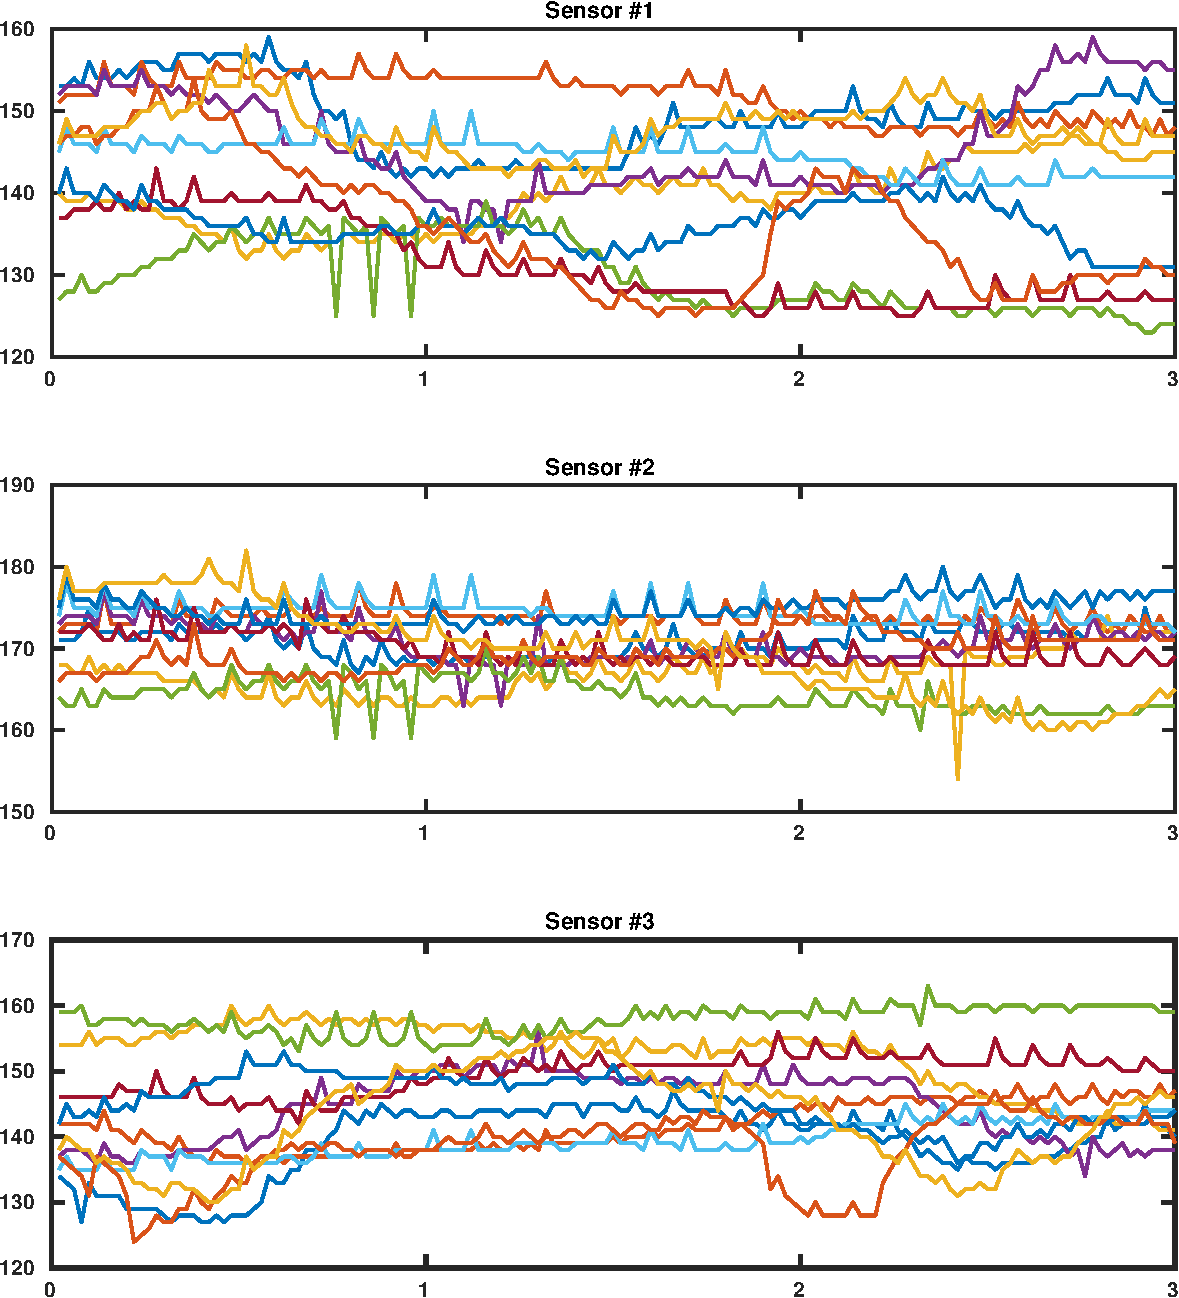
\includegraphics[width=\linewidth]{figs/stand.pdf}
%	\caption{Signals of pressure sensors embedded in the left insole when a performer is standing still. Different colours indicate different attempts for the same performer. This shows the large variation of the signal even for the same user performing the same pattern.}
%	\label{fig:stand}
%\end{figure}

The onboard chip uses the technology of Bluetooth Low Energy and sends the pressure information to other processing devices (such as a smart phone). 
Each sensor returns an integer value within the range of [0, 255] to indicate the magnitude of the foot pressure. 
The sampling frequency of the pressure information is 50Hz and the transmission frequency from the onboard chip is 10Hz. 

The training and testing of the classifier is conducted on a server computer with Intel Core i7 (six cores), 16G memory and NVidia GTX 1080Ti. 
The server computer receives the sensor data, conducts the prediction and sends the results to the VR helmet.
All data are transmitted based on TCP protocol.
A unity3D application is developed to render the virtual scene on Pico Goblin, which is an all-in-one VR device with Qualcomm Snapdragon 820 CPU and 3G memory. 
\footnote{All source code and dataset of this work can be found in the supplementary file.}

%\subsection{List of Interaction}
%We identify a list of behaviours of real humans, which are automatically recognized with our algorithm and applied to manipulate the virtual scene. The list of behaviours include stand, walk forward/backward, run, jump, slide left/right. This list is determined by conducting a pilot user study to evaluate a broad range of interactions.

\subsection{Selection of Foot Gestures}
Foot gestures, as proxy for walking-in-place, have been extensively investigated in existing works \cite{yan2004new, wendt2010gud, feasel2008llcm, bruno2013new,nilsson2016walking,nilsson2018natural}.
An elicitation study was performed to provide thorough understanding of foot gestures which are linked with the corresponding actions in three conditions: standing up in front of large display, sitting down in front of a desktop display and standing on a projected surface \cite{felberbaum2018better}.
% Our work plans to provide a wide range of locomotion skills in VE: walking forward/backward, running, jumping, sliding left/right.

Researchers define \emph{Referents} \cite{felberbaum2018better} as common actions of an avatar in VE, which our proposed gestures (in RW) are planned to trigger.
The selected referents are based on existing works and set as: walking forward/backward, running, jumping, sliding left/right \cite{lee1998control,felberbaum2018better}.

We follow the mapping from gestures to \emph{referents} as proposed in a most recent work \cite{felberbaum2018better} (shown in Figure~\ref{fig:gestures}).
% The elicitation study is set-up following the paradigm in the state-of-the-art study \cite{felberbaum2018better}, but extends it to the scenario when the user is wearing a VE helmet, with no constraints on a limited horizontal surface.
In the existing work \cite{felberbaum2018better}, participants are confined on a limited horizontal surface, which implies the use of walking-in-place.
Different from this work, we decide to offer two choices to walk forward in the VE.
One option is real walking (Figure~\ref{fig:gestures}(a)), which ensures the most realistic locomotion experience and is suitable for scenarios with sufficient space.
Another option is walking-in-place (Figure~\ref{fig:gestures}(b)), which is suitable for real environments with limited space.
This hybrid approach offers users flexibility to choose real walking when the perceived immersion is preferred and the size of physical space allows, but walking-in-place when there is no sufficient physical space. 
It is worth noting that the focus of this work is to develop a pattern classifier to identify each gesture, instead of exploring the best gestures to trigger the corresponding referents.
Selections of alternative gestures can be seamlessly integrated into the workflow of our method.



%10 participants, with an average age of 21.6 and the standard deviation (SD) of 3.20, are recruited in this pilot study. 
%Each participant is asked to rate their familiarity of Virtual Reality from 1 to 5 (Table~\ref{tab:scale}).
%The average score for such familiarity is 3.28, with the SD of 1.05.
%We believe this group of participants is appropriate for such an assessment task, since they have moderate understanding and experience of VR applications, but not influenced by the conventional mode of VR interaction.
%
%\cite{felberbaum2018better}
%
%\begin{table}[!htp]
%	\def\arraystretch{1.25}
%	\centering
%	\begin{tabular}{C{1cm}p{7cm}}
%		\hline
%		Score & Description of Criteria       \\
%		\hline \hline
%		1 & Never heard of VR concept/application/device    \\
%		2 & Have heard of VR but no hands-on experience  \\
%		3 & Have hands-on VR experience (<= 2 times)  \\   
%		4 & Have hands-on VR experience (> 2 times) \\
%		5 & Experienced user of VR applications, or engaged in related development and research\\
%		\hline               
%	\end{tabular}
%	\caption{\label{tab:scale}Questionnaire of user familiarity of interactive VR applications. }
%	% For detailed description, please refer to supplementary document.}
%\end{table}



%
%The experiment result (Figure~\ref{fig:pilot_result}) shows that in-place interaction receives lower rating in forward, backward, left and right movements.
%The common characteristics of these patterns are to use body inclination to trigger the corresponding command (Figure~\ref{fig:pilot_inplace}).
%One user describes it as 'awkward' to push the insole in order to move in the virtual scene, because such an action violates the direct intuition of moving their feet. 
%Since the pressure distribution cannot be accurately controlled and the sensor data may be noisy, users sometimes need to perform so large body inclinations that he/she looses the balance.
%Pushing the insole for a long time also leads to fatigue on the leg and foot muscles.
%However, the choice of in-place move outperforms free move in terms of running and jumping.
%In the mode of free move, users expressed their concern about colliding with objects in the real world since both patterns involve large ranges of dynamic movements with their eyes being blocked by the VR device.
%Therefore, in order to allow users to run and jump in the real world, we need a considerably large space. 
%This may not be possible given the limited space in many scenarios. 
%Some works tackled this problem with the technique of redirected-walking \cite{dong2017smooth}, by adjusting the orientation of the trajectory with minor extent so that users rotate in the real world without actual sensing.
%This allows exploration in a wider range of VE, given the same size of the real world.

%\begin{figure*}
%	\centering
%	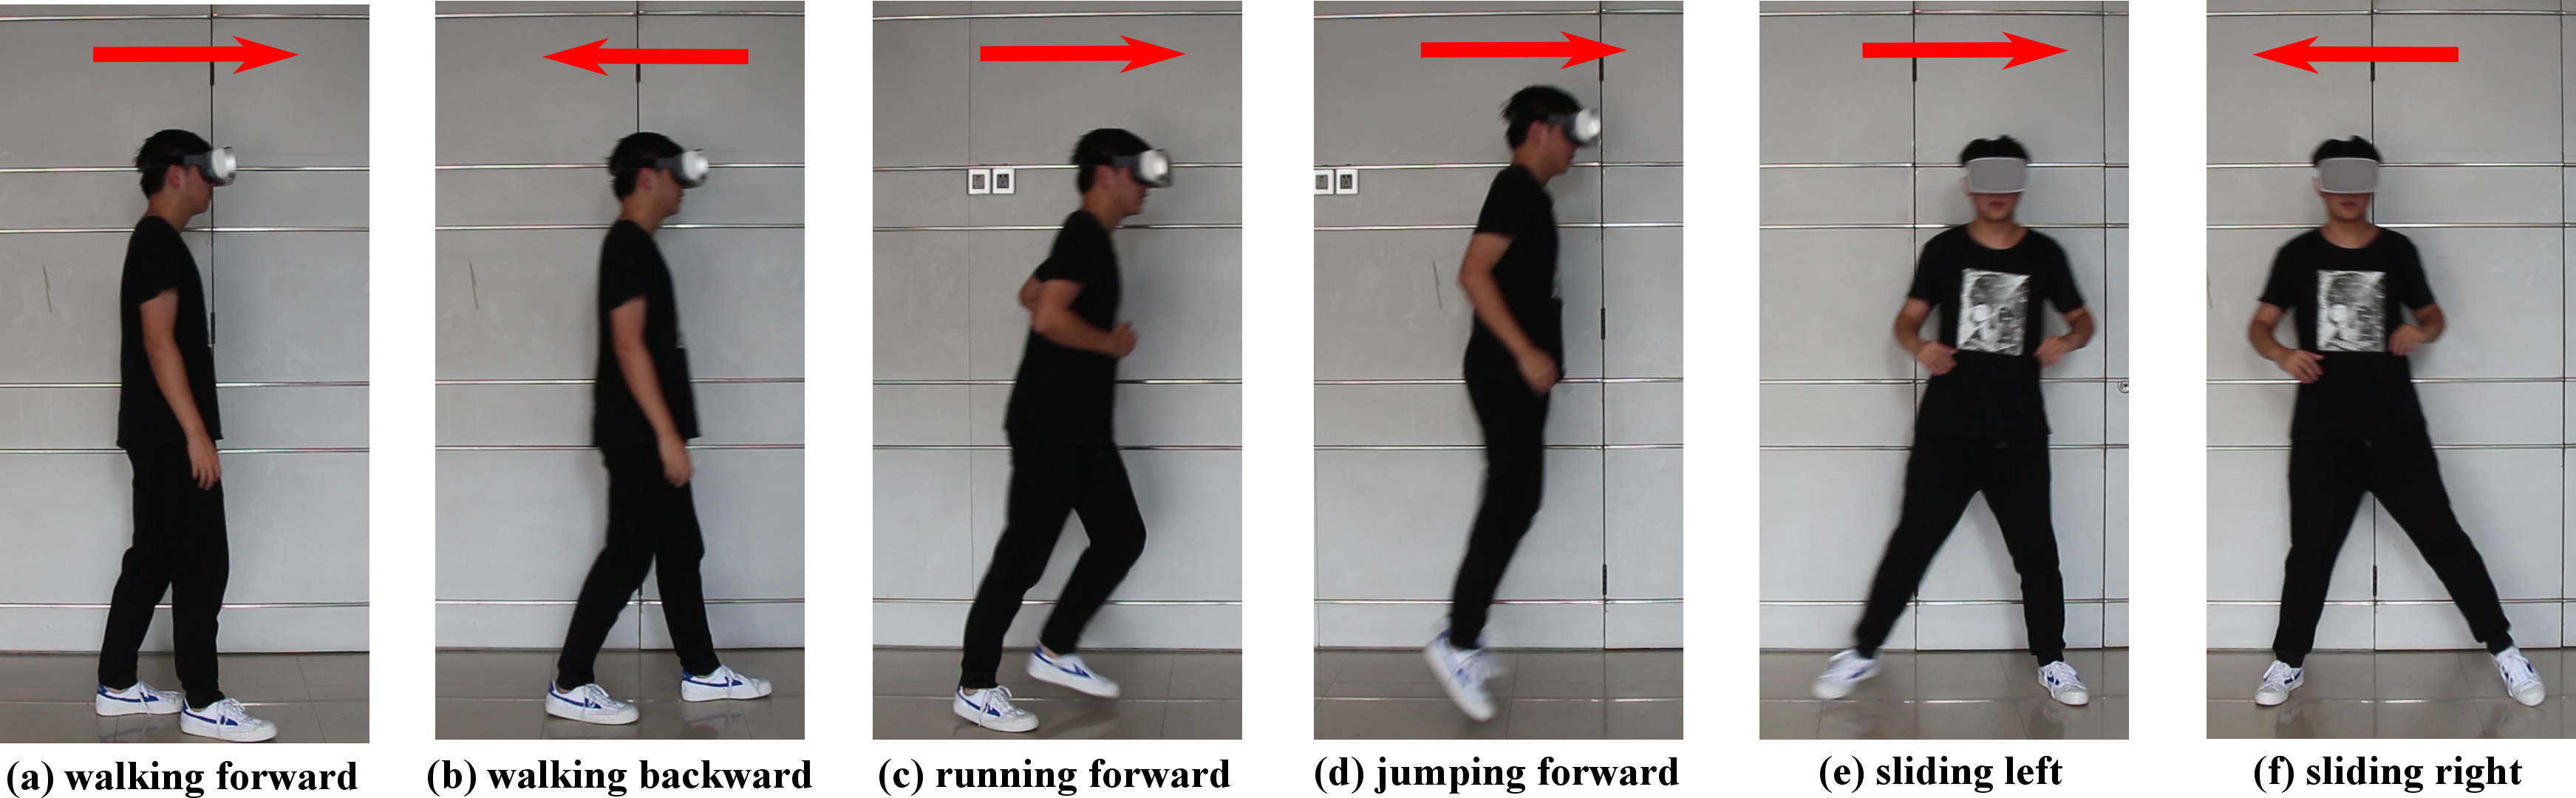
\includegraphics[width=\textwidth]{figs/pilot_real.png}
%	\caption{Motion patterns of free move to trigger the same actions as in-place move.}
%	\label{fig:pilot_real}
%\end{figure*}



%\begin{figure}
%	\centering
%	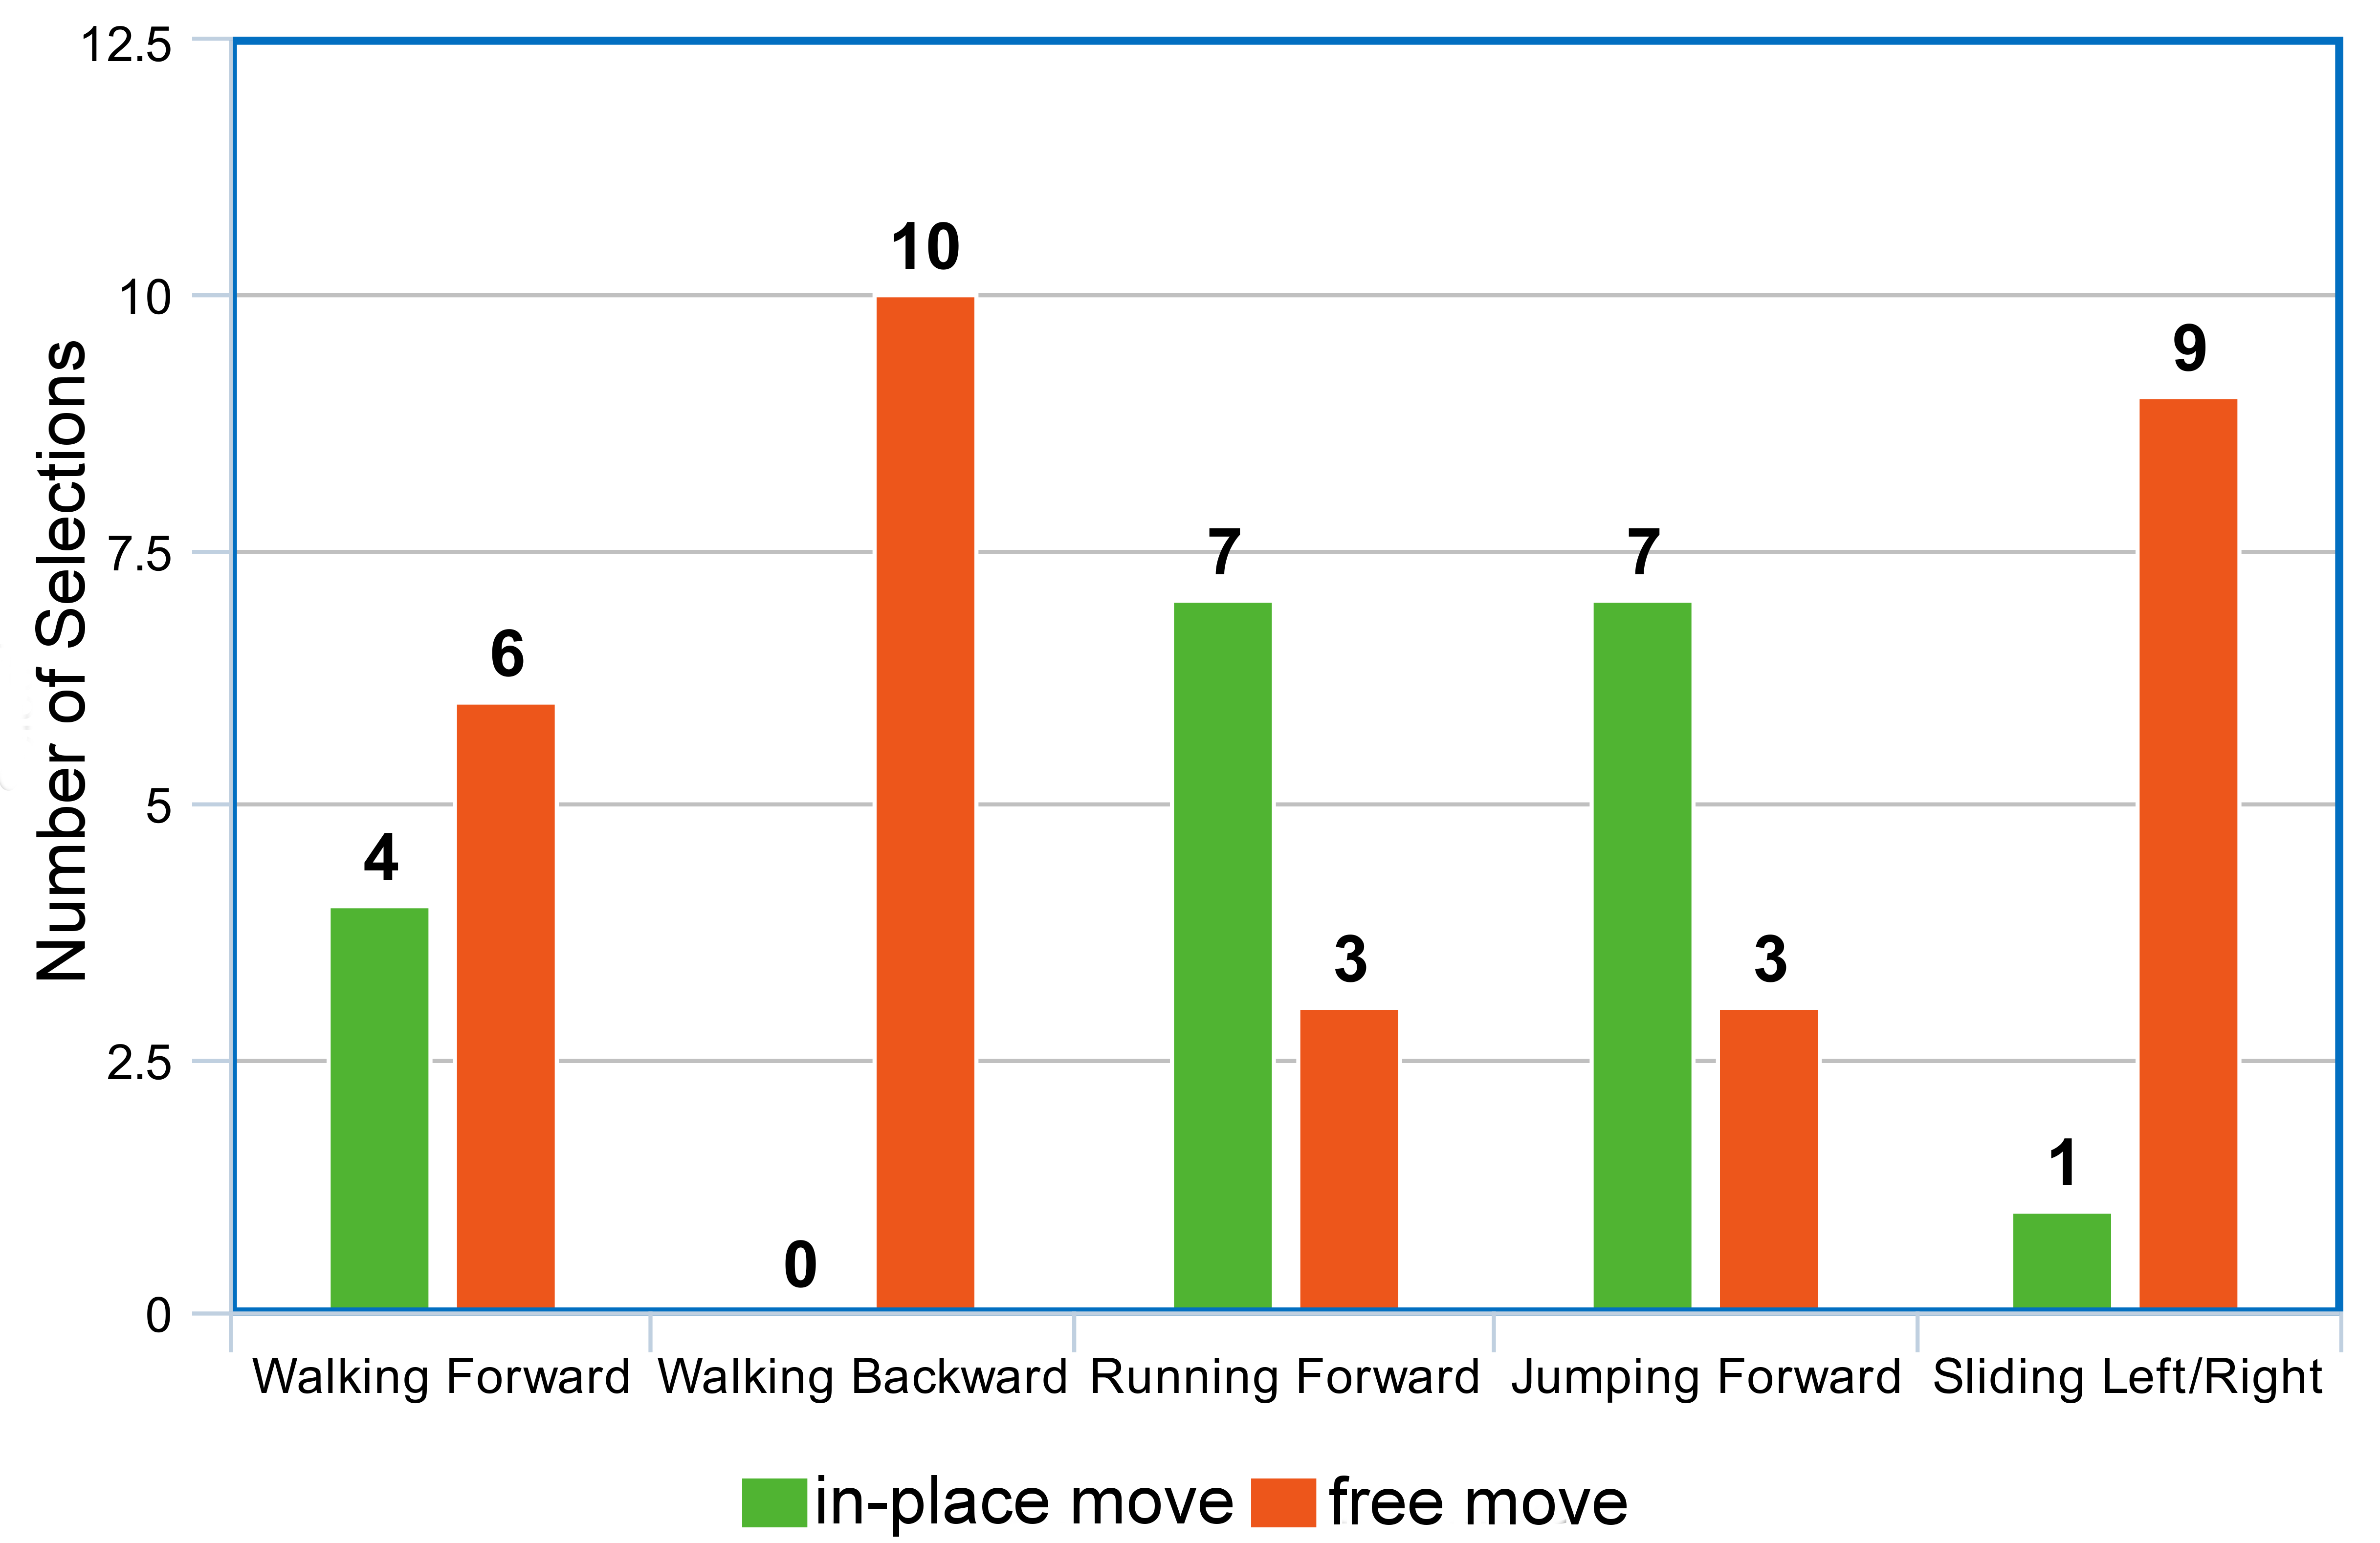
\includegraphics[width=\linewidth]{figs/pilot_result.png}
%	\caption{Comparison of in-place and free moves in pilot study.}
%	\label{fig:pilot_result}
%\end{figure}

\section{Gesture Classifier Training}
\label{sec:training}
\subsection{Data collection}

\begin{figure}
	\centering
	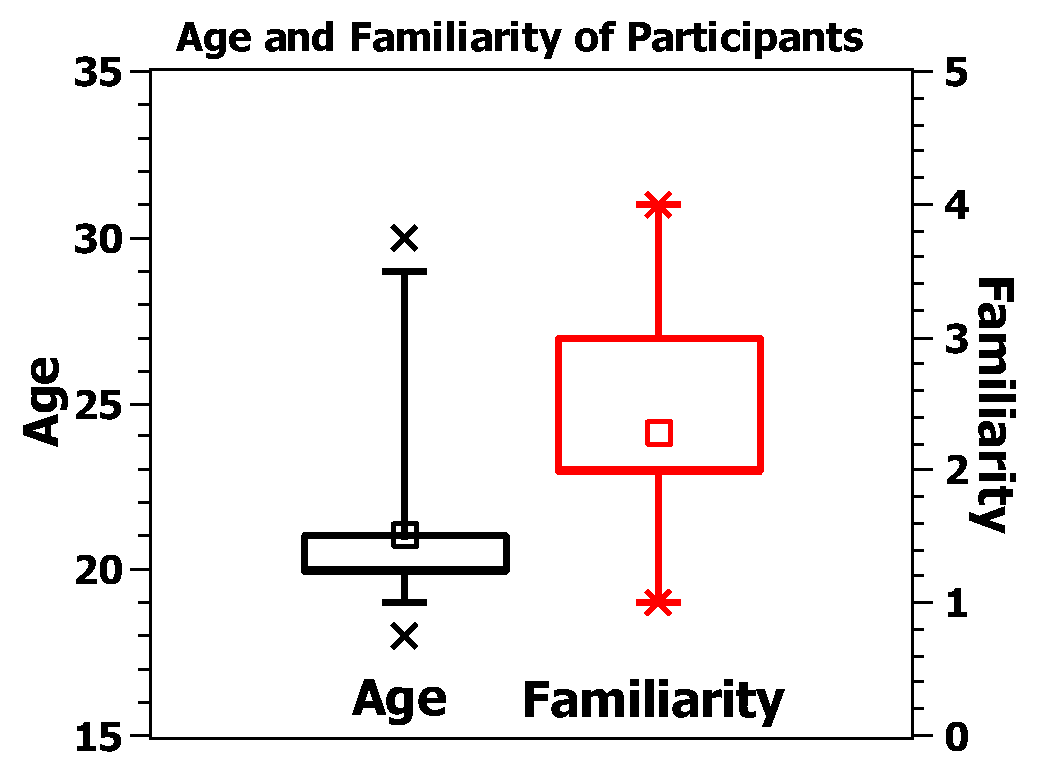
\includegraphics[width=\linewidth]{figs/training_users.pdf}
	\caption{Age and familiarity score of participants in the session of data collection.}
	\label{fig:training_users}
\end{figure}

\paragraph{Participants} Experiments have been carried out with a group of 38 volunteers with an average age of 21.34 and the standard deviation of 3.45.
The age distribution is plotted in Figure~\ref{fig:training_users}.
The participants are students and faculties from our university, ranging from first-year undergraduate to associate professors.
The distribution of shoe sizes and male/female is presented in Table~\ref{tab:shoesize}.
Participants involved in the stage of data collection are not recruited for latter validation studies.

\begin{table}[!htp]
	\def\arraystretch{1.25}
	\centering
	\begin{tabular}{C{1.5cm}C{2.0cm}C{1.5cm}C{1.5cm}C{1.5cm}}
		\hline
		Shoe Size (US) & Num. of Participants & Num. of Female & Total Duration \\
		\hline \hline 
		6  & 13 & 13 & 699.5 \\
		7.5 & 12 &7  & 714.45 \\
		8.5 & 13 &0  & 780.5 \\
		\hline               
	\end{tabular}
	\caption{\label{tab:shoesize}Number of participants and length of durations in the process of data collection.  The unit of duration is minutes in the collected dataset.}
\end{table}

Each participant is asked to rate their familiarity of Virtual Reality from 1 to 5 (Table~\ref{tab:scale}).
The average score for such familiarity is 2.28, with the SD of 0.82.
We believe this group of participants is appropriate for this task, since they have moderate understanding and experience of VR applications, but not influenced by the conventional techniques of VR interaction.

\begin{table}[!htp]
	\def\arraystretch{1.25}
	\centering
	\begin{tabular}{C{1cm}p{7cm}}
		\hline
		Score & Description of Criteria       \\
		\hline \hline
		1 & Never heard of VR concept/application/device    \\
		2 & Have heard of VR but no hands-on experience  \\
		3 & Have hands-on VR experience (<= 2 times)  \\   
		4 & Have hands-on VR experience (> 2 times) \\
		5 & Experienced user of VR applications, or engaged in related development and research\\
		\hline               
	\end{tabular}
	\caption{\label{tab:scale}Questionnaire of user familiarity of interactive VR applications. }
	% For detailed description, please refer to supplementary document.}
\end{table}


\paragraph{Procedures} 
Each participant performed eight activities (standing, real walking, walking-in-place, walking backward, running, jumping, sliding left and right) wearing the smart insoles and the VR helmet.
The helmet displays a virtual environment of open square which allows users to navigate around.
At the beginning of the experiments, participants are informed of the experiment purpose.
Participant is presented with a virtual scene which guides him/her to perform each activity individually.
The activities are performed in short duration (10 seconds) with repeated attempts.
Participants are instructed to familiarize with the system before the start of data collection.
This pre-collection step costs around 2 minutes.
The capture process is conducted in a sufficiently large space, which allows the users to perform these activities in a non-stop attempt.
A timer is presented to the participant on the VR screen, informing him/her the elapsed time since the start of the current capture session.
A participant is free to terminate the capture process at any time if he or she feels tired.
Participants are given sufficient rest time during collection sessions.
The collected data from each session are automatically uploaded to our server and manually annotated with the corresponding gesture label.
The complete collection for each user costs around one hour, including the rest time for participants.




%\begin{figure*}
%	\centering
%	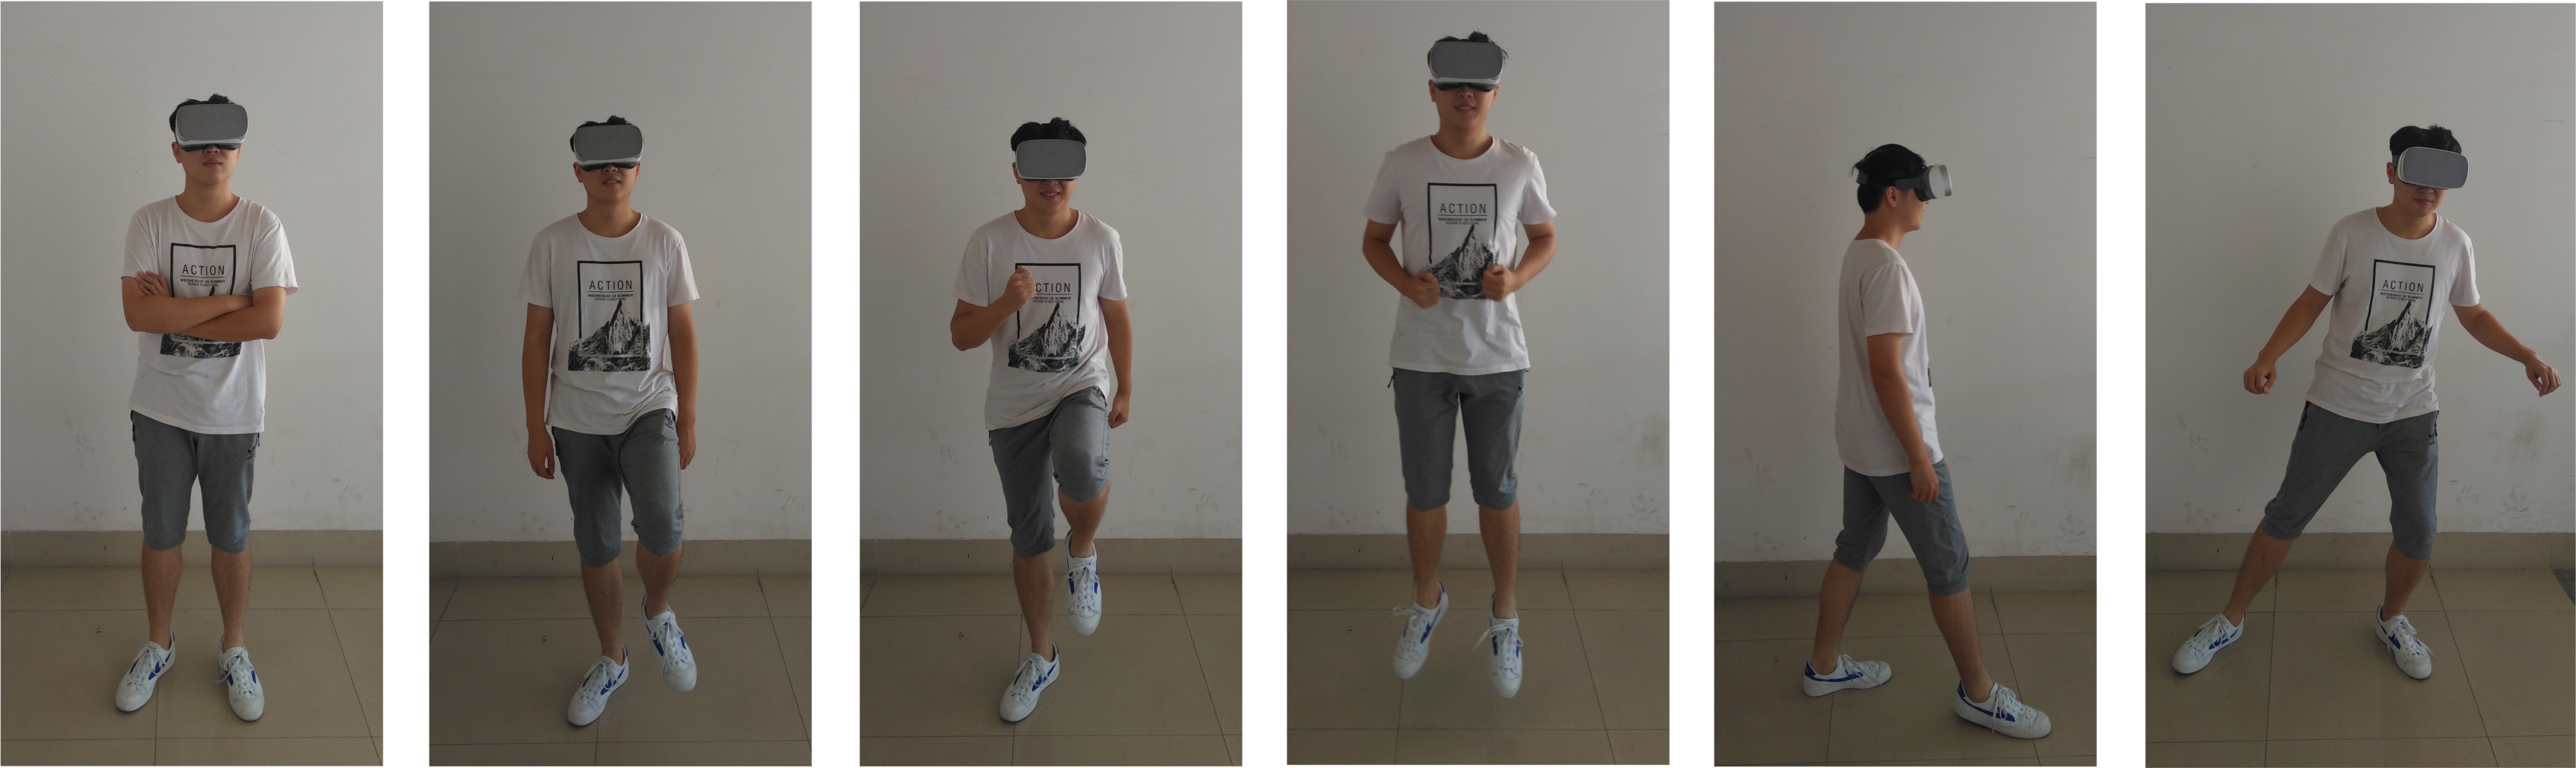
\includegraphics[width=\linewidth]{figs/six_tasks.png}
%	\caption{Image capture of users in the procedure of collecting training data. From left to right: standing, walking, running, jumping, walking backward, sliding left/right.}
%	\label{fig:six_tasks}
%\end{figure*}
%
%\subsubsection{Post-processing of the data}
%The pressure signals were pre-processed by applying noise filters and then sampled in fixed-width sliding windows of 1.0 sec and 50\% overlap. 

%\begin{table}[!htp]
%	\def\arraystretch{1.25}
%	\centering	
%	\begin{tabular}{C{2cm}C{3cm}C{3.5cm}}
%		\hline
%	Interaction Pattern	& Num. of \newline testing samples & Num. of \newline training samples \\
%		\hline\hline
%		jumping           & 2712           & 13863           \\
%		\hline
%		running           & 2724           & 13437           \\
%				\hline
%		standing          & 2724          & 14580           \\
%				\hline
%		walking \newline in situ  & 2709           & 13656           \\
%				\hline
%       walking \newline forward  & 2241           & 11481           \\
%				\hline
%		walking \newline backward & 2790           & 13371           \\
%				\hline
%		walking \newline left     & 2850           & 15195           \\
%				\hline
%		walking \newline right    & 2847           & 14487           \\
%				\hline
%		total             & 21597          & 110070          \\
%		\hline
%	\end{tabular}
%	\caption{\label{tab:action}List of interaction patterns and the corresponding statistics on testing and training datasets.}
%\end{table}

\begin{table}[!htp]
	\def\arraystretch{1.25}
	\centering	
	\begin{tabular}{C{2.8cm}C{2.3cm}C{2.3cm}}
		\hline
		Pattern	& Num. of \newline testing samples & Num. of \newline training samples \\
		\hline\hline
		standing          & 2724           & 14580           \\
		%\hline
		real walking          &    2241       & 11481    \\		
		walking in place  & 2709           & 13656          \\
		%\hline
		walking backward & 2790           & 13371           \\
		jumping           & 2712           & 13863           \\
		%\hline
		running           & 2724           & 13437          \\
		%\hline		
		%\hline
		sliding left     & 2850           & 15195           \\
		%\hline
		sliding right    & 2847           & 14487           \\
		%\hline
		total             & 21597          & 110070          \\
		\hline
	\end{tabular}
	\caption{\label{tab:action}Statistics of selected foot patterns in testing and training datasets. All data are provided as the supplementary file of this publication.}
\end{table}

\begin{figure*}[!htbp]
	\centering
	\begin{subfigure}{0.43\linewidth}
		\centering
		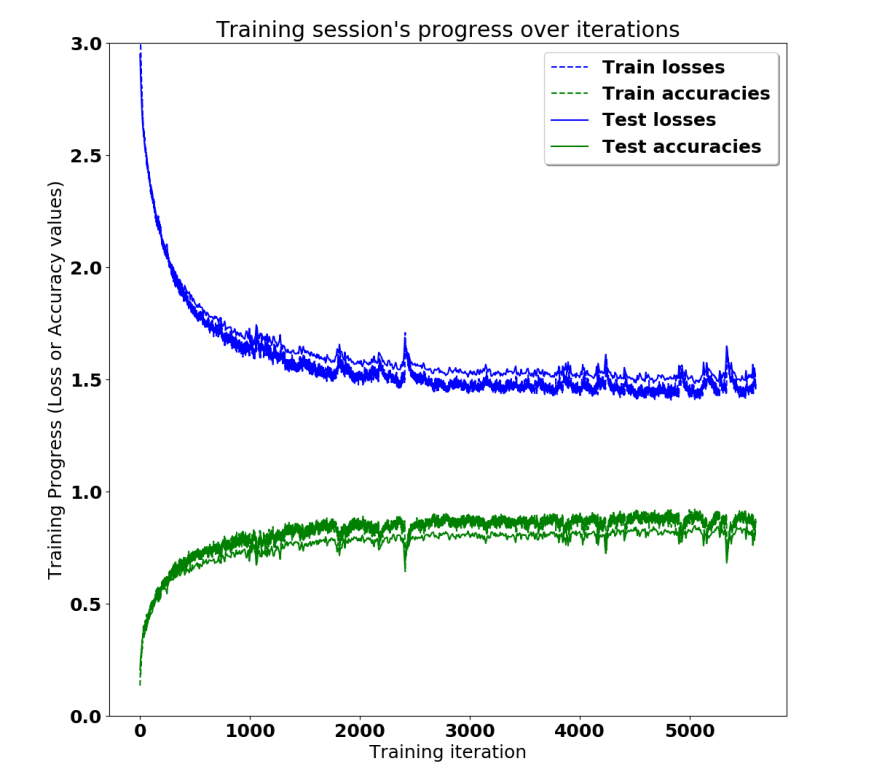
\includegraphics[width=\linewidth]{./figs/accuracy_loss.png}
		\caption[]{\label{fig:accuracy_loss} Participant In Action
		}
	\end{subfigure}
	~
	\begin{subfigure}{0.5\linewidth}
		\centering	
		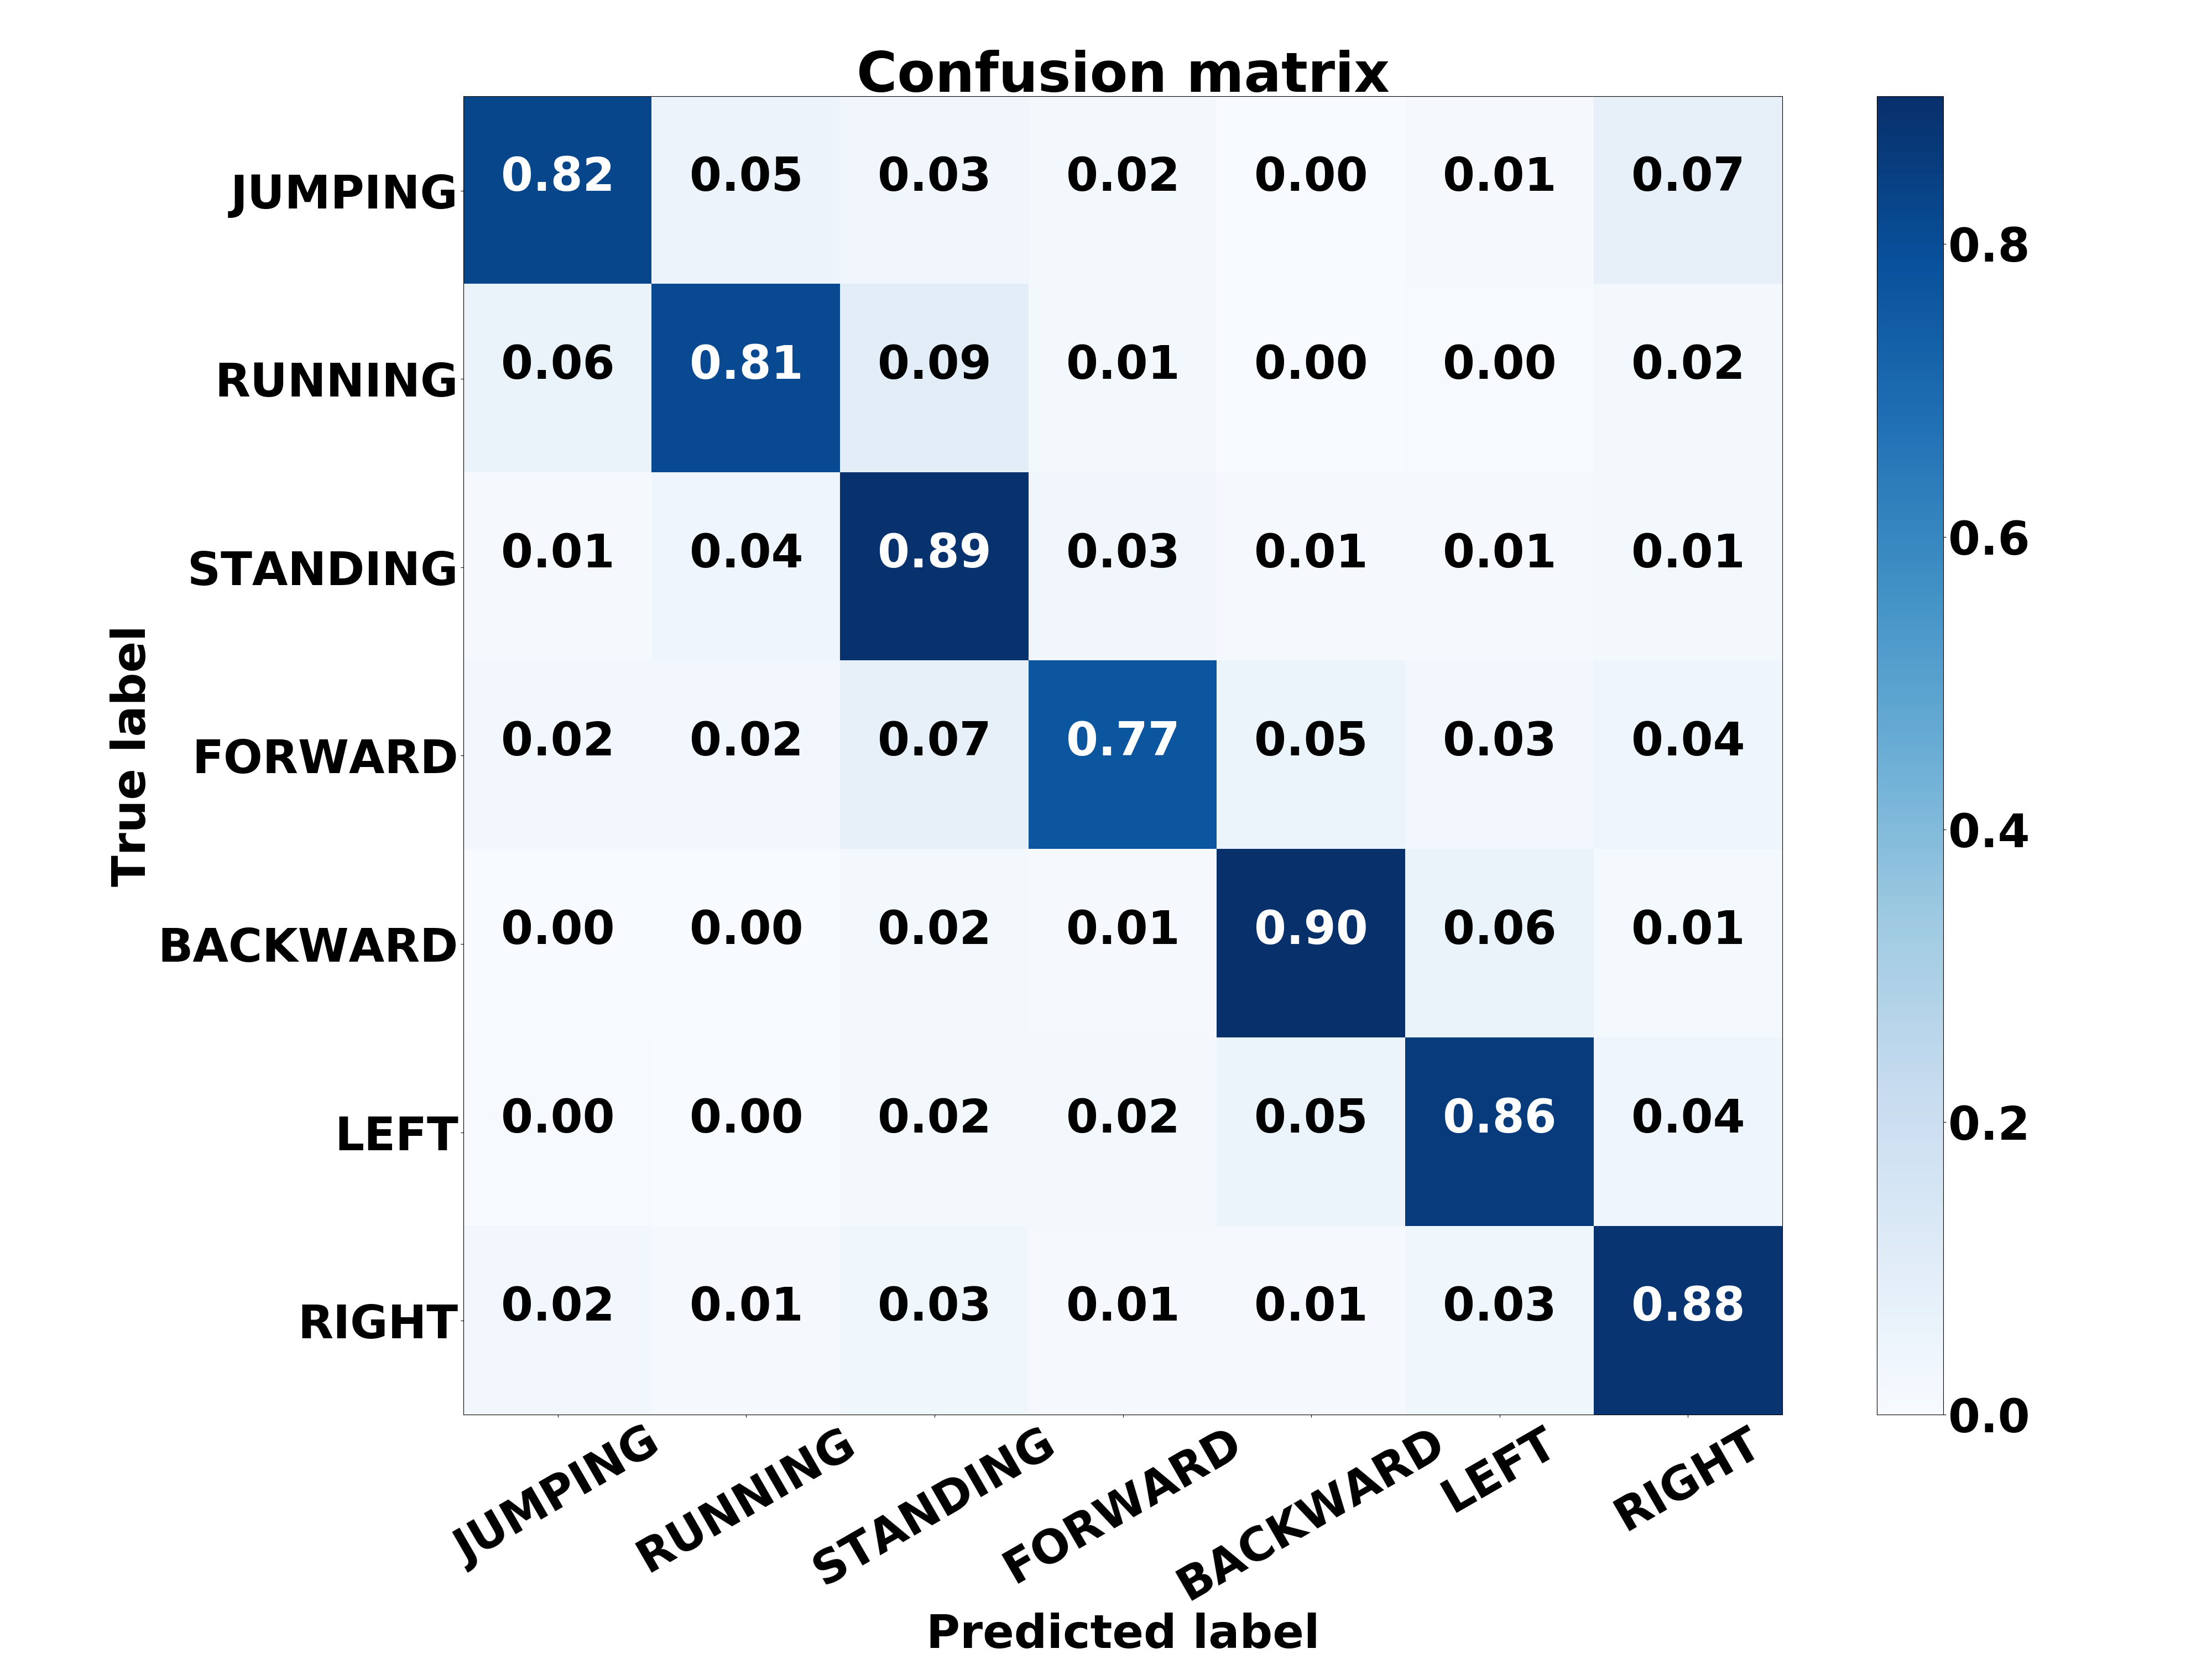
\includegraphics[width=\linewidth]{./figs/confusion_matrix.jpg}
		\caption[]{\label{fig:confusion_matrix} First-person View
		}
	\end{subfigure}			
	\caption[]{\label{fig:training_lstm}
		Results from training the standard LSTM classifier (sequence size $\mathbf{S}$=100, equivalently 2 seconds). (a) Losses and accuracies for both training and testing dataset. (b) Normalized confusion matrix for the selected behavior patterns.
	}
\end{figure*}

\subsection{The standard LSTM Classifier}
\paragraph{Data Processing}
For each participant, we normalize the corresponding data with the maximal sensor-specific pressure value in the collection dataset for individual participants. 
This technique is designed to neutralize the effect of different body weights of users.
Our method works directly with noisy input and no filtering is required for the collected data.
After that, the time-series data are divided into samples, each of size $\mathbf{N}\times\mathbf{S}$, where $\mathbf{N}$ is the number of sensors and $\mathbf{S}$ is the sequence size of each sensor signal. 
It is worth noting that the sequence size $\mathbf{S}$ critically affects the prediction accuracy.
Multiple sequences sizes, between 10 to 100, are tested in our method (see detailed analysis in Section~\ref{sec:compare_performance}).

The complete dataset has been randomly partitioned into two sets on the level of individual participants.
For shoe sizes of 6, 7.5, 8.5, 11, 10, 11 participants respectively are selected as the training data and the rest participants as the testing data. 
The separation between training and testing datasets on the individual level allows us to prove the effectiveness of our classifier to extend to individuals who are not included in the session of data collection.
The statistics of the collected database are presented in Table~\ref{tab:action}.

\paragraph{Training the Standard LSTM Classifier}
Long Short-Term Memory (LSTM) is an improved sub-category of Recurrent Neural Network and could avoid the problem of vanishing gradient. 
We take a sample matrix $\mathbf{X}$ of size $\mathbf{N}\times\mathbf{S}$ as network input, and its corresponding label vector $\mathbf{Y}$ as network output.
%The network output is a probability vector for classification. 
The network model has 3 LSTM layers, each of 64 hidden units, with 1 fully-connected layer as the output. 
The network loss function is defined as:
\begin{equation}
    \mathcal{L} = || \mathbf{Y} - \mathbf{Y}_p ||^2
\end{equation}
where $\mathbf{Y}_p$ is the prediction from the network.
We use the Adam Optimizer with the learning rate of 0.0025, the batch size of 1500. 
Compared with conventional methods in classification of time-series data like Hidden Markov Model (HMM) and Dynamic Time Warping (DTW), we do not require manual feature engineering and avoid the problem of user-specific parameters. 
Further comparison with existing classification methods can be found in Section~\ref{sec:compare_performance}.
%Further, with the method of neural network, we can effectively adapt to different users with no further adjustments.

Figure~\ref{fig:accuracy_loss} shows the loss and accuracy for both training and testing datasets. 
The learning fast converges to an optimal solution after 1000 iterations and reaches an accuracy of 70\%, which costs around 20 minutes. 
% By this time, the accuracies for training and testing datasets are both around 0.7. 
As the learning progresses, the final accuracy reaches over 85\% for both training and testing datasets. 
The result shows that the accuracy of the testing dataset is close to the training dataset, which implies that the problem of over-fitting is avoided and our method is capable of generalizing to variations from individual users.

%\begin{figure}[!htp]
%	\centering
%	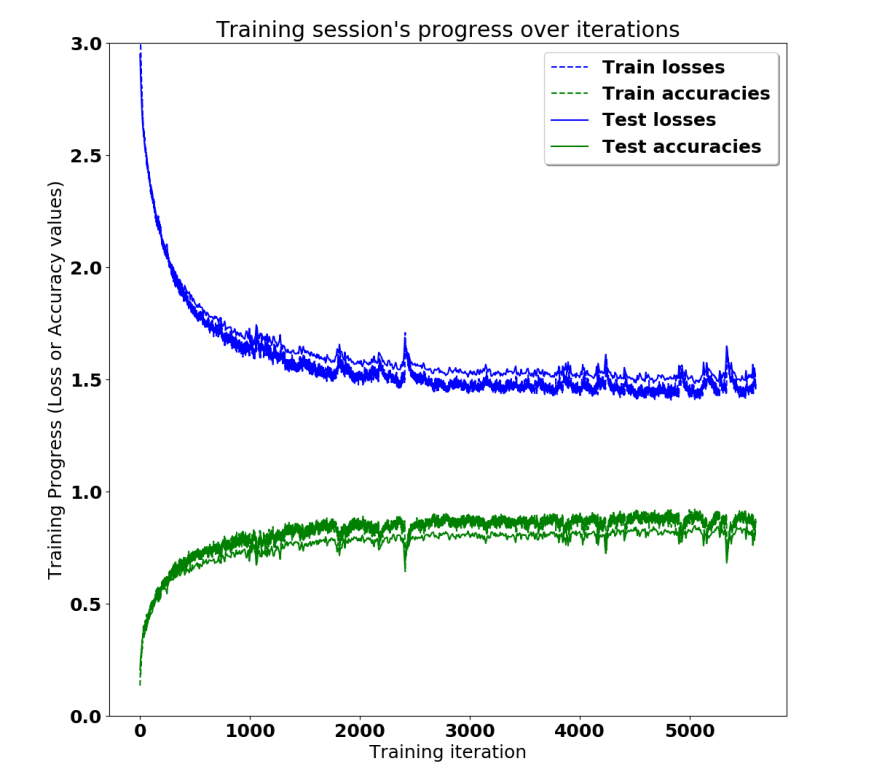
\includegraphics[width=\linewidth]{figs/accuracy_loss.png}
%	\caption{Losses and accuracies for both training and testing dataset. This plot is generated using the training and testing dataset of shoe size 6 with the sequence size of 100.}
%	\label{fig:accuracy_loss}
%\end{figure}

Figure~\ref{fig:confusion_matrix} shows the normalized confusion matrix of different behavior patterns in the mode of walking-in-place, with a sequence size of 100 (2 seconds). 
The result shows that the action of walking forward (in the mode of walking-in-place) is recognized with the lowest accuracy of 77\%.
Walking forward is incorrectly labelled as standing (7\%) and walking backward (5\%).  
This error is caused by the similarity of these foot patterns.
It is worth noting that when switching to the mode of real-walking, the accuracy improves to 81\%.
Real walking allows users to lift off their feet for an extended duration of time and thus reduces the possibility of mis-labelling as standing.
Meanwhile, the patterns of standing, walking backward and sliding left/right are recognized with a rather high accuracy of over 85\%.
The accuracy is further improved with the novel method \acs{doctic} proposed in the following paragraphs.
%\begin{figure}[!htp]
%	\centering
%	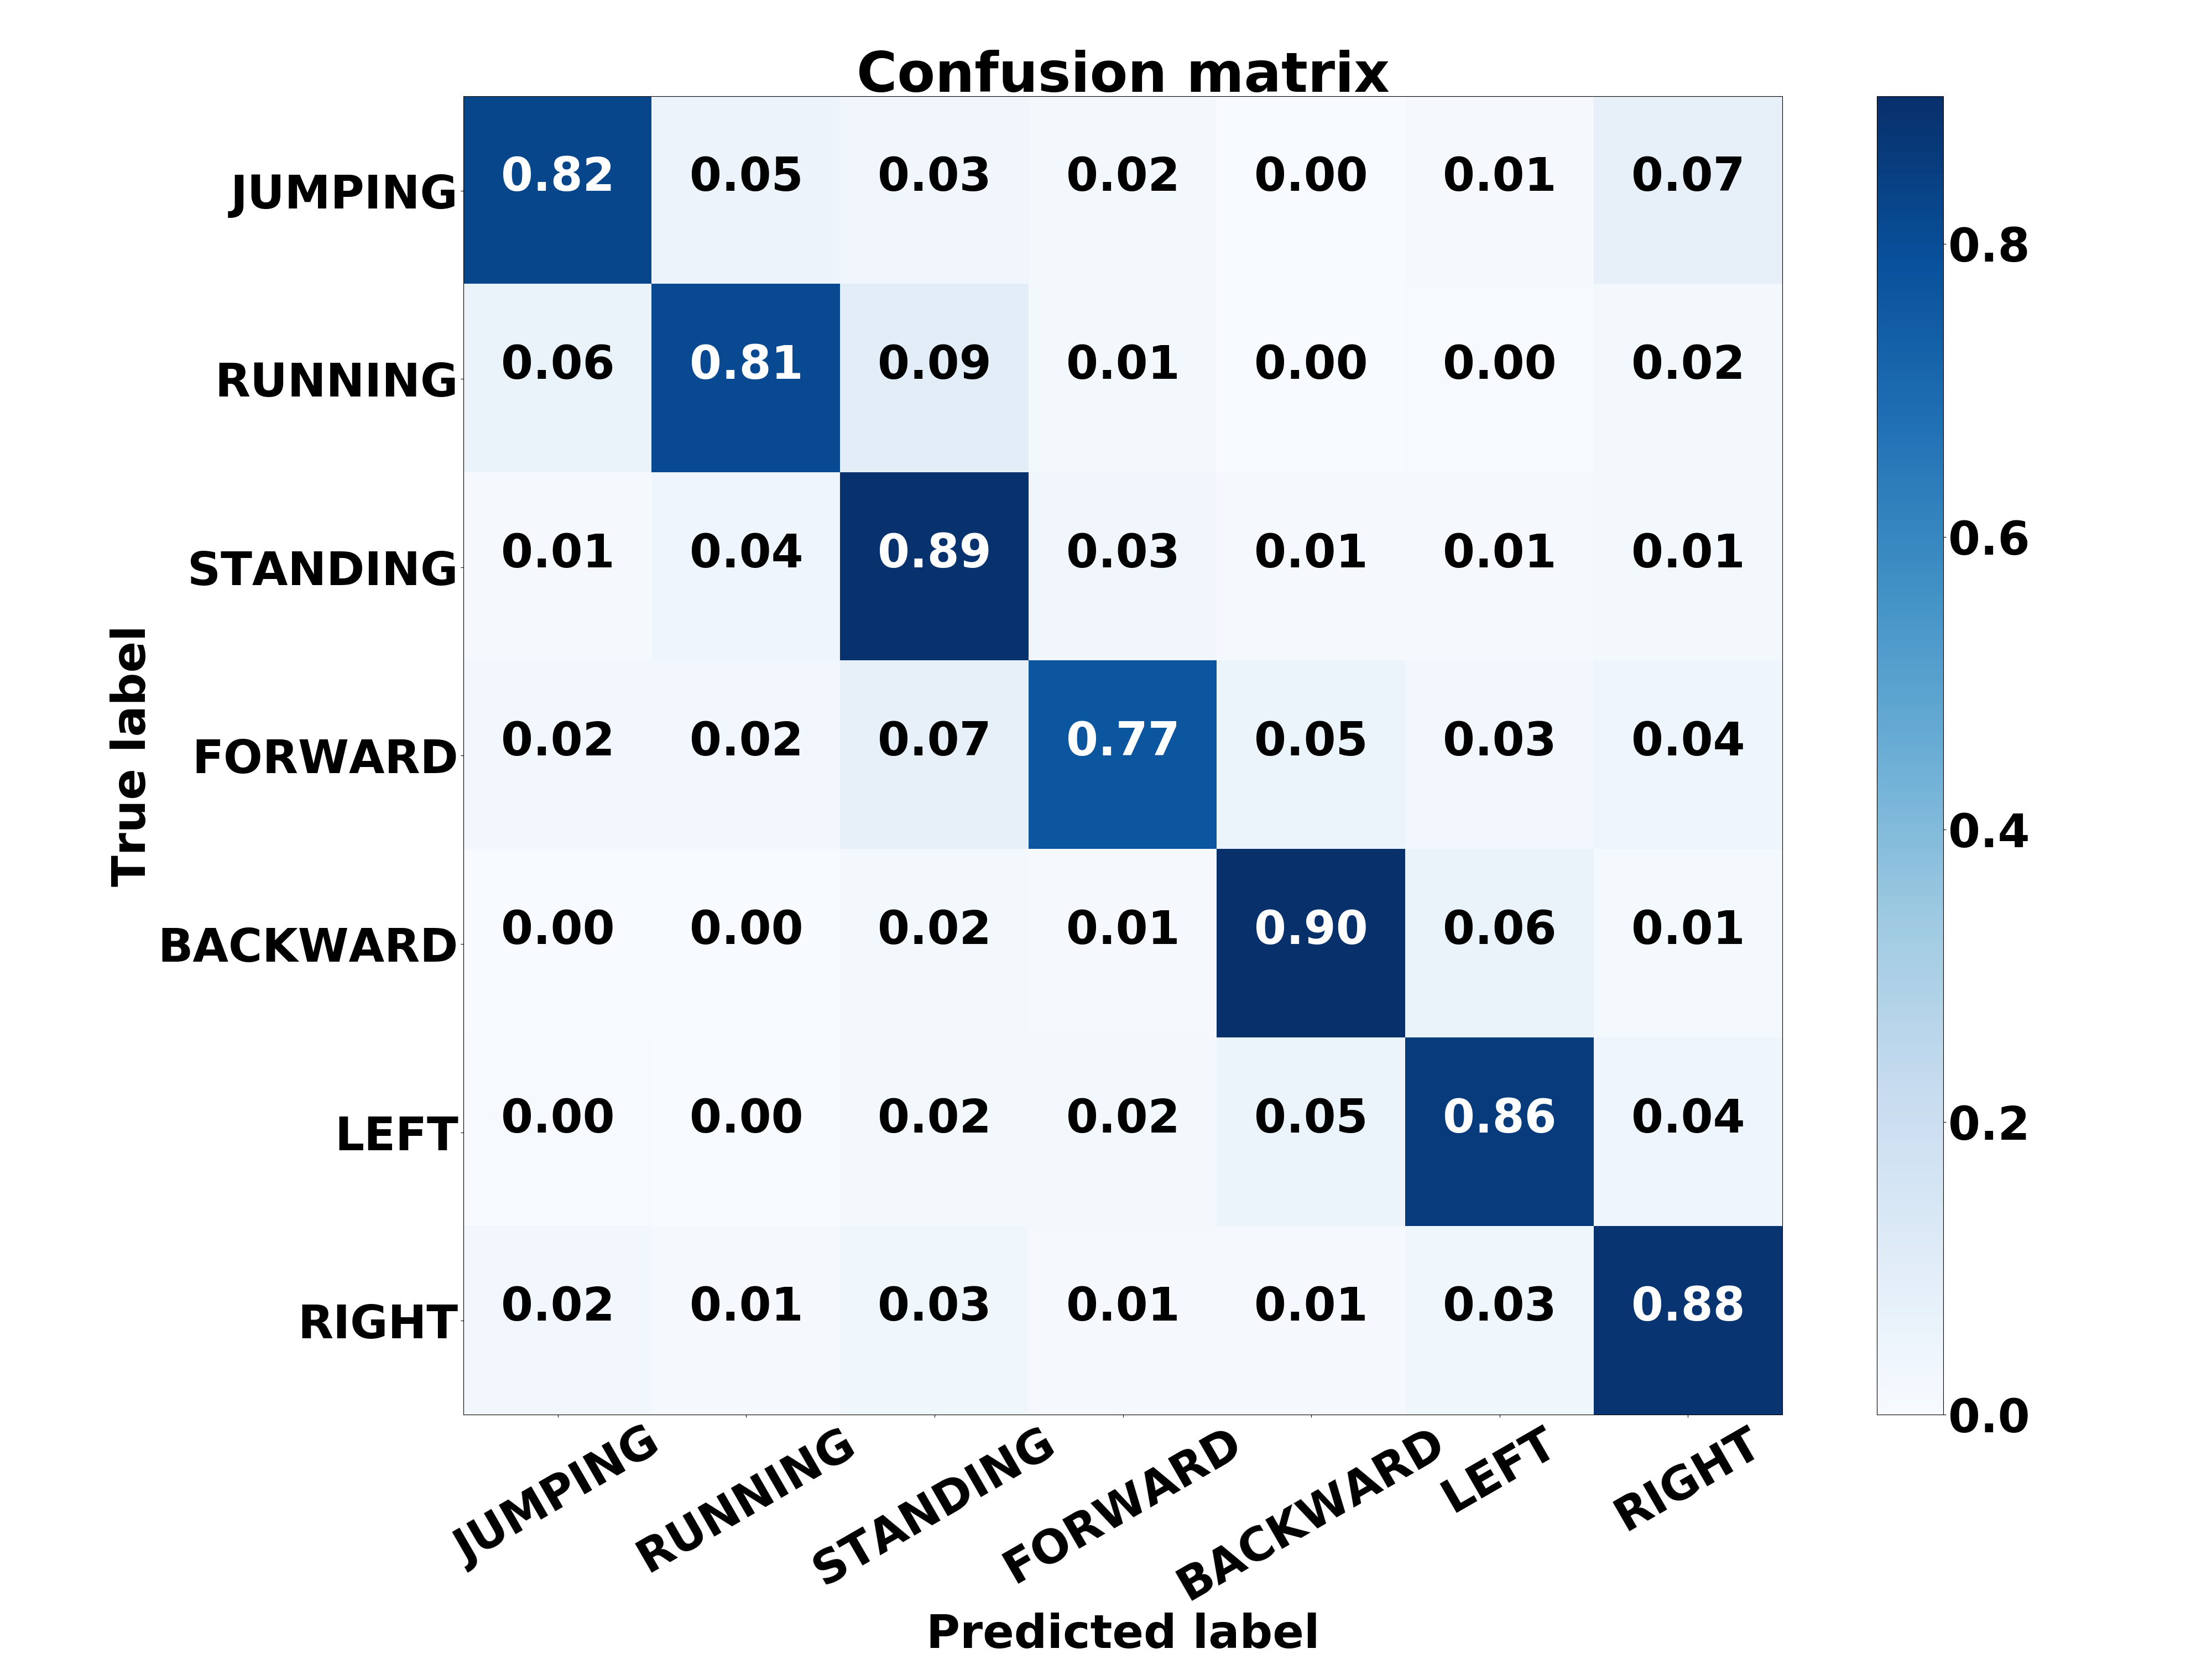
\includegraphics[width=\linewidth]{figs/confusion_matrix.jpg}
%	\caption{Normalized confusion matrix for the selected behavior patterns. This plot is generated using the testing dataset of shoe size 6 with the sequence size of 100.}
%	\label{fig:confusion_matrix}
%\end{figure}



\subsection{\acl{doctic}}
Standard \acs{lstm} can classify the motion patterns with an accuracy of $\sim$80\% given a large sequence of data (2 seconds) (Figure~\ref{fig:training_lstm}). 
This indicates that the algorithm can only correctly identify the pattern of jumping possibly after the jumping is finished.
This latency could critically lead to negative user experiences.
We propose a novel method, \acf{doctic} (Figure~\ref{fig:flowchart}), to fast predict the pattern label while improving the accuracy performance.

Our initial observation is that the forward computation of \acs{lstm} model is efficient (less than 1 millisecond).
Based on such an observation, we applied an iterative procedure to compare the predictions $\mathbf{Y}$ using the samples of sequence duration of both T and T+$\delta$T.
\begin{equation}
   T, \mathbf{Y} = \underset{T, \mathbf{Y}}{\arg} (<\mathbf{Y}_p^T> \doteq <\mathbf{Y}_p^{T+\delta T}>)
\end{equation}
We here define the operator $\doteq$ as the identification of the first element-wise equality in two vectors $<\mathbf{Y}_p^T>, <\mathbf{Y}_p^{T+\delta T}>$.
\begin{equation}
    <\mathbf{Y}_p^T> = \cup \mathbf{Y}_p^t,\ t \in [0, T]
\end{equation}
Therefore, we are searching for a pair of parameters $T, \mathbf{Y}$, which leads to the first-time equality of two predictions $\mathbf{Y}_p^T, \mathbf{Y}_p^{T+\delta T}$.
T starts from the smallest segment of 0.1 second and increases to 1 second, while $\delta$T is 0.1 second.
If the predictions from both samples reach the consensus, the algorithm returns this result; otherwise, T is increased until the consensus is made or the maximum value of T is reached.
For the latter case, the pattern with the highest probability in previous predictions is selected.

If we assume the probability distribution of the standard LSTM network as $\mathbf{P}(\mathbf{Y}|\mathbf{X})$,  the probability $\mathbf{P}^*$ from our DOCTIC method is:
\begin{equation}
\mathbf{P}^*_T(\mathbf{Y}|\mathbf{X}_T,\mathbf{X}_{T+\delta T}) = 1 - \prod_{t=0}^{T} (1 - \mathbf{P}(\mathbf{Y}|\mathbf{X}_t)\mathbf{P}(\mathbf{Y}|\mathbf{X}_{t+\delta t}))    
\end{equation}
    
%\]
%\[
%    T = \frac{log(1 - \mathbf{P}^*)}{log(1 - \mathbf{P})} \delta T
%\]
This indicates that increasing the variable T leads to a higher prediction accuracy, or clamping the accuracy with a lower threshold reduces the timecost for iterative verification.     

\begin{figure}[h]
	\centering
	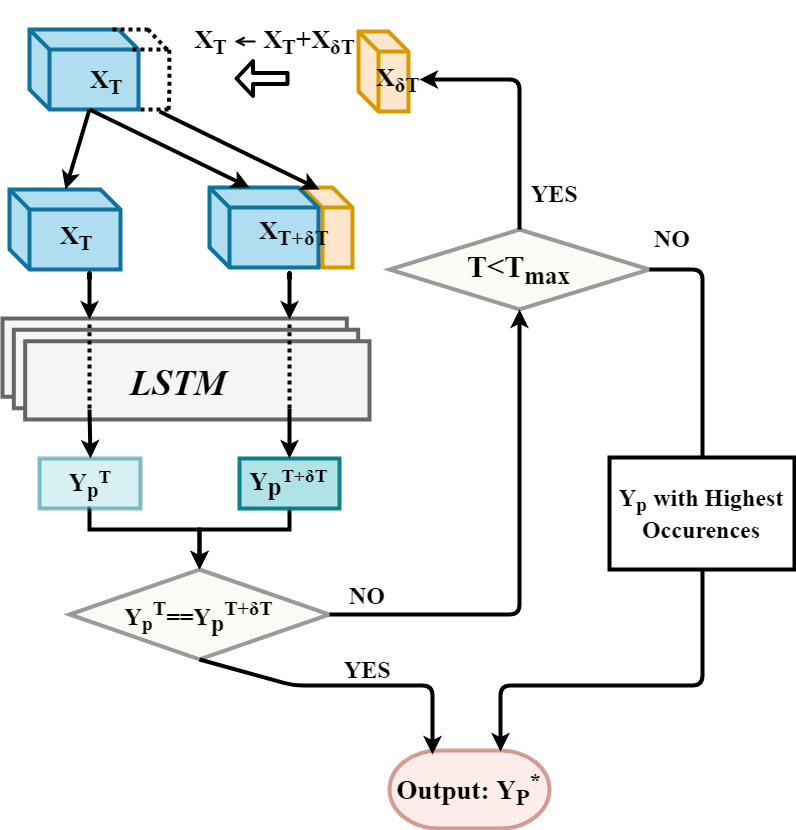
\includegraphics[width=\linewidth]{figs/flowchart.png}
	\caption{Flowchart of our DOCTIC algorithm.}
	\label{fig:flowchart}
\end{figure}


%Results show that the latency is reduced to 0.5 seconds while the accuracy is increased to over 97\%.
We train both the standard LSTM and DOCTIC classifiers for each shoe size, and the general shoe size (Table~\ref{tab:indi_size}).
The results show that the proposed \acs{doctic} method increases the accuracy by at least 10\%, in comparison to the standard LSTM method.
To reach an accuracy of 95\%, the proposed \acs{doctic} method only requires the sequence duration of 0.5 seconds.
This is significantly reduced in comparison to the sequence duration of 2 seconds of the standard \acs{lstm} method (only achieving an accuracy below 85\%).
The performance advantage is analyzed in details, in comparison to the \acs{lstm}, \acs{hmm}, \acs{dtw} methods (see Section~\ref{sec:compare_performance})).

Additionally, the results (Table~\ref{tab:indi_size}) show that training the individual classifier achieves better accuracy, over the general classifier.
We draw a conclusion that using the corresponding classifier for a specific shoe size is a direct solution to raise the accuracy.
As everyone is aware of his/her own shoe size, users are prompted to provide their shoe size when they use this application for the first time.
The file size of the network model is around 9 megabytes, which is sufficiently small to be downloaded from the remote server.
% so that multiple models can be saved on the hard disk even for an embedded system.
\begin{table}[!htp]
	\begin{tabular}{C{3cm}C{2cm}C{2cm}}
		\hline
		Shoe   Size (US) & LSTM &   DOCTIC \\
		\hline\hline
		6                                                          & 0.83   & 0.97  \\
		7.5                                                        & 0.84   & 0.94  \\
		8.5                                                        & 0.83   & 0.96  \\
		General                                                    & 0.78   & 0.88
		\\\hline
	\end{tabular}
	\caption{\label{tab:indi_size}Accuracy for training the individual classifier for different shoe sizes and a general classifier for all shoe sizes.}
	%The sequence size $\mathbf{X}$ is 100 for LSTM and 25 for LSTM\&DOCTIC.}
\end{table}


\section{User Study}
\label{sec:userstudy}
We conduct the user study to evaluate the proposed interaction technique of using foot gestures for virtual locomotion, in particular comparing against the benchmark of using joystick.

\paragraph{Participants} 10 volunteers (5 males and 5 females) with an average age of 21.25 and SD of 3.54 are recruited in this study. 
The average familiarity of VR (measured with Table~\ref{tab:scale}) is 2.50 and the SD is 0.85. 
%This familiarity score is consistent with the one from the stage of data collection.
\begin{figure}[h]
	\centering
	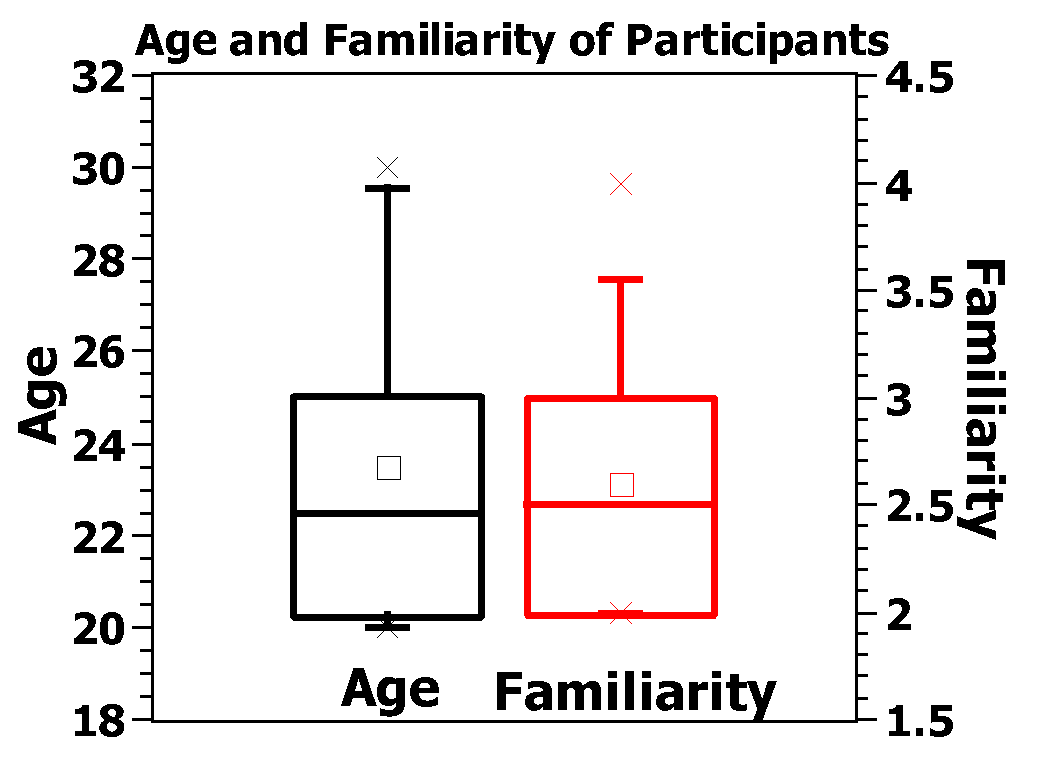
\includegraphics[width=\linewidth]{figs/testing_users.pdf}
	\caption{Age and familiarity score of participants in the session of validation.}
	\label{fig:testing_users}
\end{figure}

\paragraph{Procedures}
We developed the application on the VR helmet with the Unity framework.
A virtual track (Figure~\ref{fig:track}), with separate segments indicating users to perform the corresponding patterns, is set up to verify our hypothesis that the accuracy and latency of DOCTIC are acceptable in real-world scenarios. The track area is 86.4$\times$52.8 square meters and the sequence of various action prompts is randomly generated for each individual to eliminate the influence of the order. In particular, 8 hurdles are arranged  (on the left side in Figure~\ref{fig:track_layout}) so that the participant needs to jump over the hurdles consecutively. For the segment of walking backward, the viewpoint is rotated 180 degrees so the virtual character walks backward and returns to the starting point. 
The track begins at the red dot in Figure~\ref{fig:track_layout}, and terminates at the same position. 
The room in RW is sufficiently large to allow the participant to walk backwards with no safety concern of object collision. In this scenario, participants are free to choose either real walking or walking-in-place on their own preference to achieve the forward walking.

\begin{figure}[!htpb]
	\centering
	\begin{subfigure}{0.45\linewidth}
		\centering
		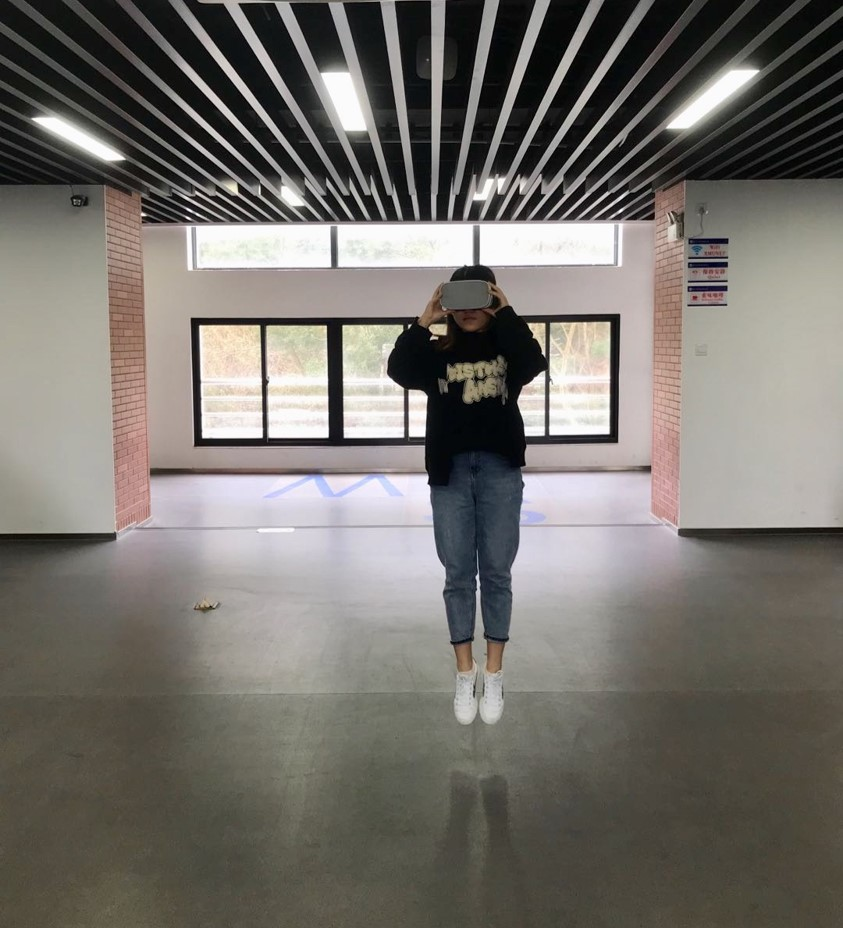
\includegraphics[width=\linewidth]{./figs/track_real.jpg}
		\caption[]{\label{fig:track_real} Participant In Action
		}
	\end{subfigure}
	~
	\begin{subfigure}{0.45\linewidth}
		\centering
		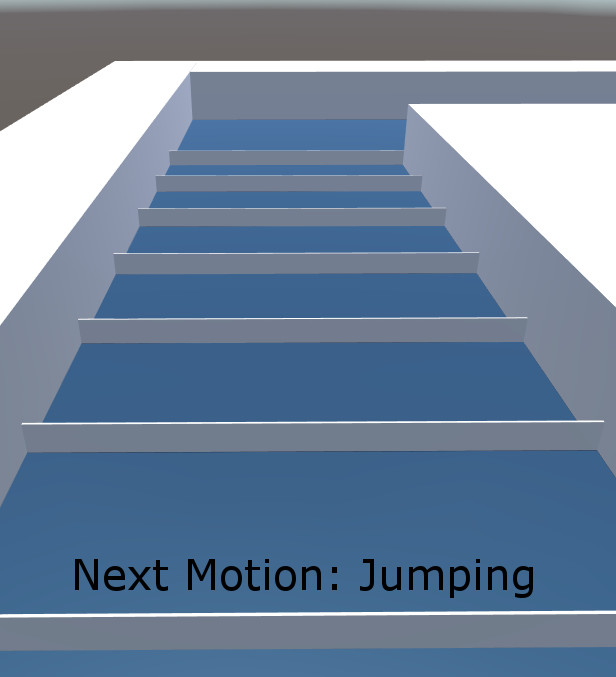
\includegraphics[width=\linewidth]{./figs/track_close.jpg}
		\caption[]{\label{fig:track_close} Jumping Section
		}
	\end{subfigure}
	~
	\\
	\begin{subfigure}{\linewidth}
		\centering	
		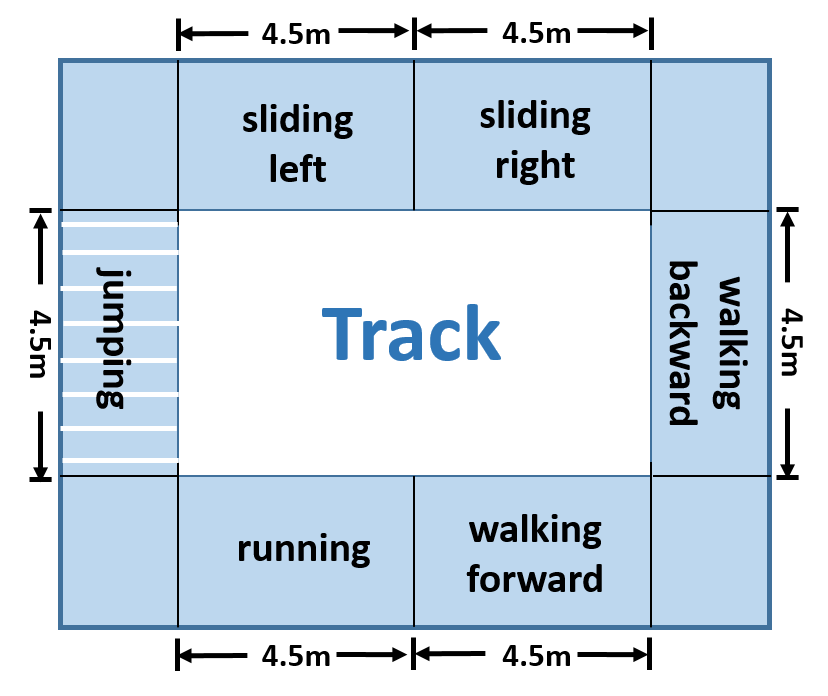
\includegraphics[width=\linewidth]{./figs/track_layout.png}
		\caption[]{\label{fig:track_layout} Top View
		}
	\end{subfigure}			
	\caption[]{\label{fig:track}
		Interactive demo of navigating in a virtual track.
	}
\end{figure}

Firstly, participants are guided to perform these series of gestures with the joystick as the benchmark, requiring no physical involvement. In addition, they repeat the same task utilizing smart insoles as interaction technique with either the standard LSTM or DOCTIC model  without knowing the exact classification algorithm.
% After the experiment, participants rate the accuracy and latency in their perception separately against the benchmark. 
When running the real-time application, users are guided to perform a few actions (walking-in-place, running-in-place and jumping-in-place) before starting the main application.
At this stage, the algorithm estimates the 'maximal' pressure value used for the purpose of weight normalization.
These parameters are dynamically updated as a user is engaging in this application.
After experiencing the above experiments, participants rate the interestingness, engagement, easy to learn and easy to use using a 5-point Likert scale for joystick and smart insoles respectively (1-bad experience, 5-great experience).

\paragraph{Analysis} In terms of user's subjective preferences about the two interaction techniques, we evaluate the difference of the two interaction techniques for the four aspects (interestingness, engagement, easy to learn and easy to use) using one-way ANOVA. 
The results show that in terms of interestingness (F=11.54, p<10$^{-2}$) and engagement (F=35.53, p<10$^{-3}$), users have higher preference of smart insoles in comparison to the joystick, while in terms of easy to learn (F=1.25, p=0.279) and easy to use (F=1.76, p=0.202), users do not show significant differences in the two interaction techniques.
%Combining with the analysis of mean and standard deviation, it is safe to say that the traditional joystick based interaction is inferior to our insoles based one for evaluation indicators of interestingness and engagement. 
Some participants suggested that smart insoles provide a better immersive and enjoyable experience resulting from the physical involvement.
%, which explains why the joystick based interaction dims in comparison with smart insoles based one under the user evaluation. 
Based on the above results, we believe that our method provides a promising solution to real-time VR interaction.

%Participants report over 85\% success of DOCTIC while LSTM only achieves less than 70\% success which is intolerable for users. Besides the subjective evaluation from users, 
We also collect the mis-labelled actions for each segment showing a mean accuracy of 82\% for our DOCTIC method and 65\% for standard LSTM. 
As for the latency, our DOCTIC model also distinctly outperforms the standard LSTM. 
Most participants have complained about the unacceptable delay in the process based on the standard LSTM model especially in the segment of jumping. Nevertheless, some comments for DOCTIC are: "I cannot feel the latency for most of the time". 
% We also ask participants about their preferences and feelings about these two interaction modes, joystick based and smart insoles based. Some of them claim that smart insoles provide a better immersive and interesting experience resulting from the physical involvement. Figure 12(b), where 8 out of 10 participants choose our proposed method over the standard joystick, has revealed that the joystick based interaction dims in comparison with smart insoles based. Based on the above results, we believe that our method provides a promising solution to real-time VR interaction.


\begin{figure}
	\centering
	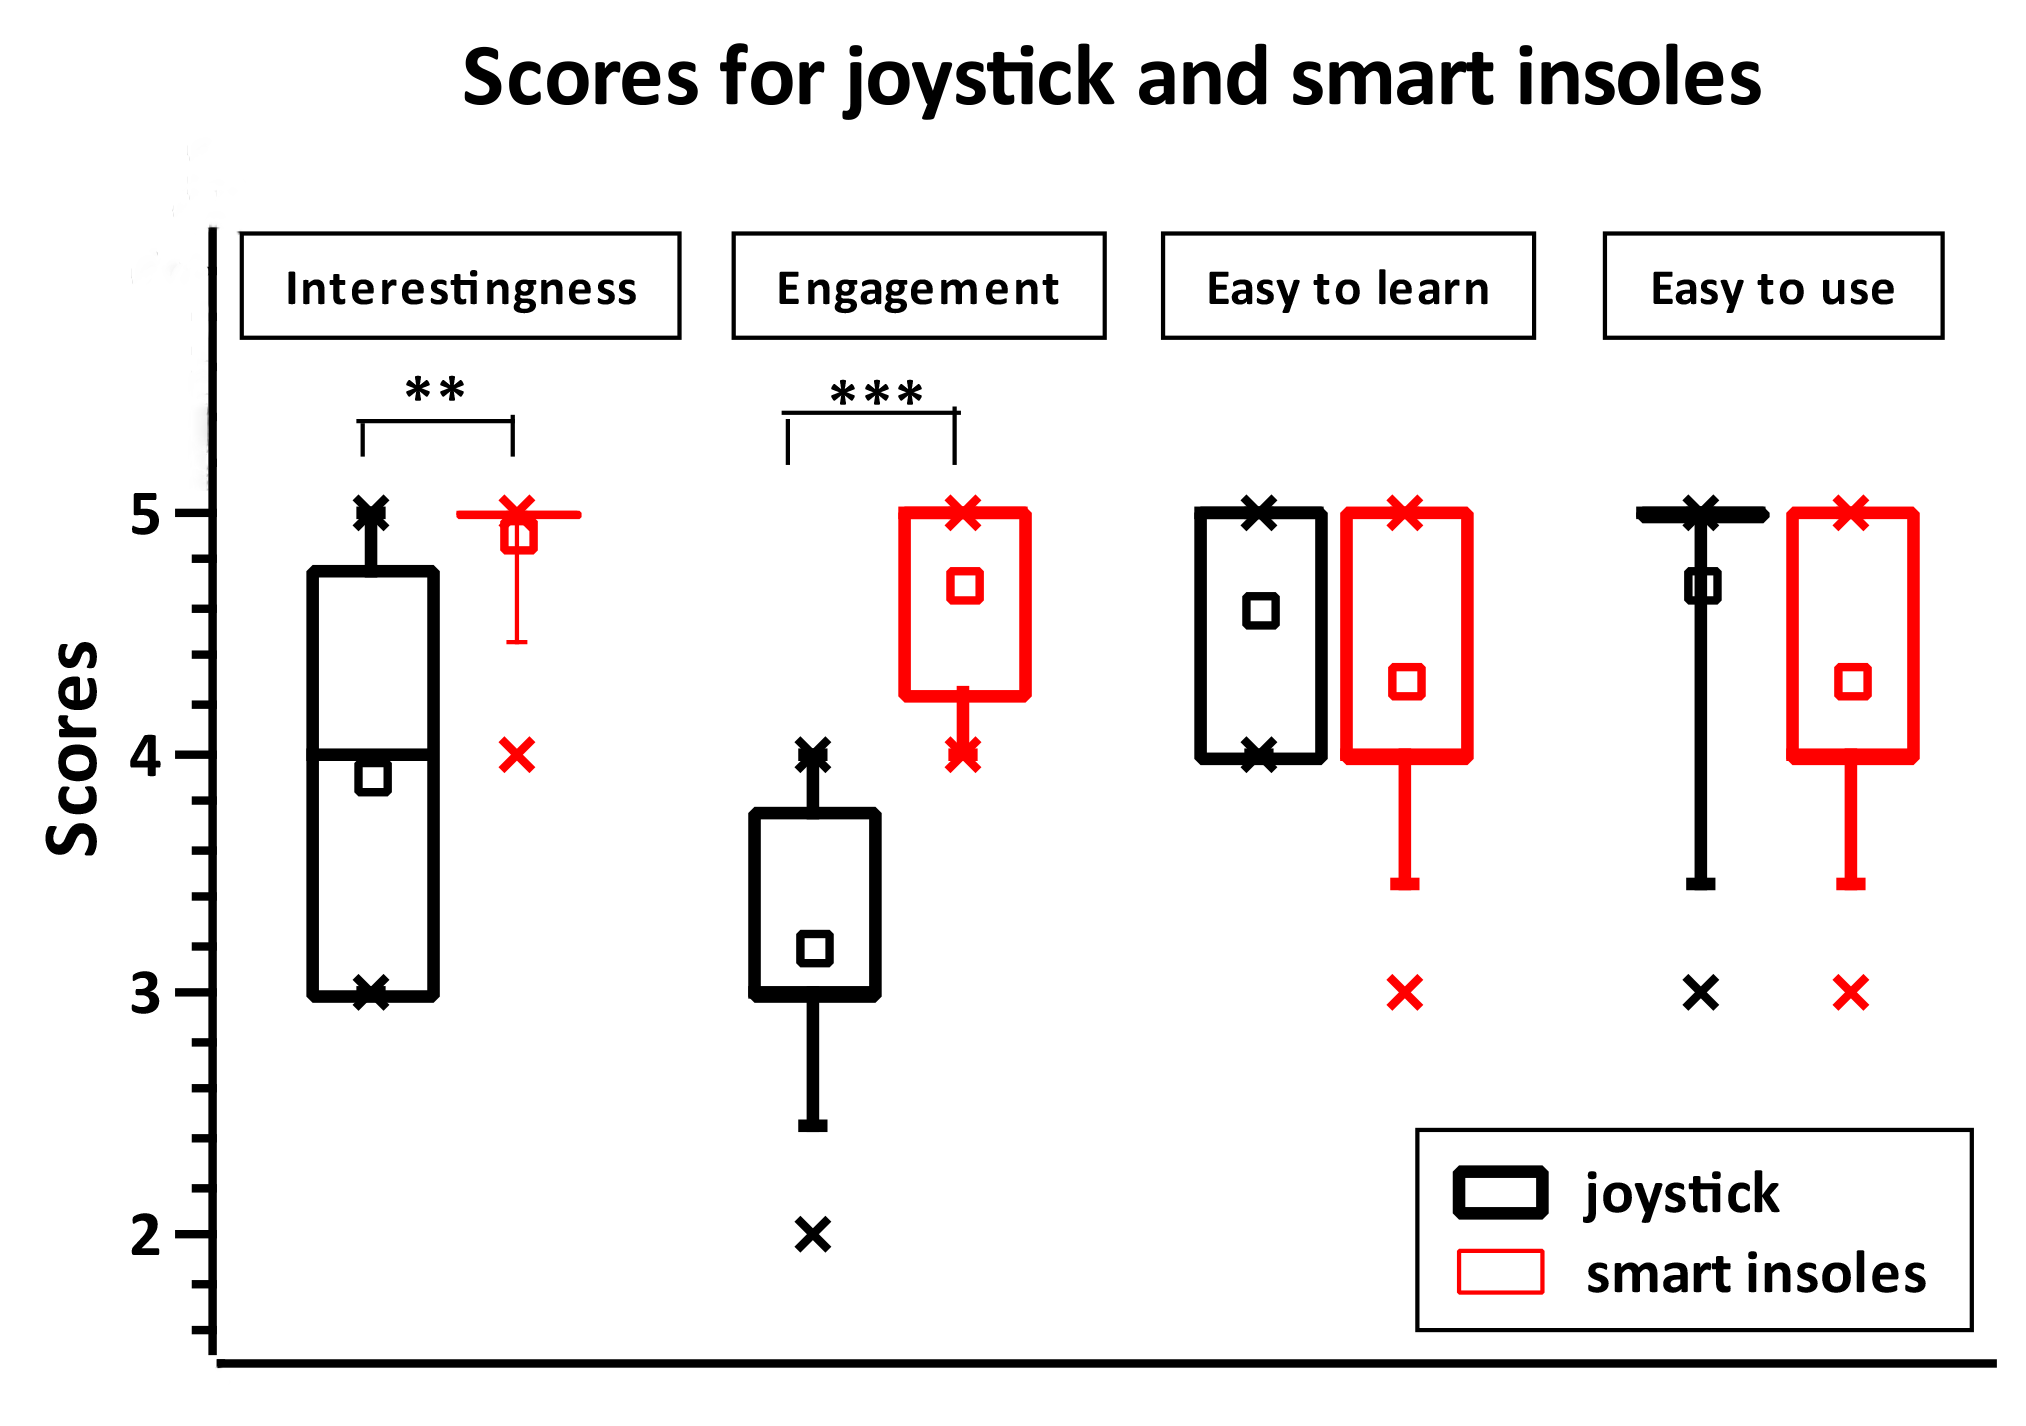
\includegraphics[width=\linewidth]{figs/scores.png}
	\caption{Result from our user experiments.(* indicates the level of significance between the two interaction techniques.)}
	\label{fig:final_scores}
\end{figure}

% We deem that the normalization process is conductive to the apparent gap of accuracy between theory and practice. Reasons are as follows. The only post-processing procedure when preparing the training dataset is to normalize the data with the maximal sensor-specific value for individual participants.
% When running the application in real-time, it is challenging to estimate such 'maximal' pressure values within a short time interval.
% The current solution is to set up a starting stage when users are guided to perform a few actions before starting the main application.

% Accordingly, how to fast estimate such parameters is critical to maintain a high accuracy at the initial stage of the application.

\begin{figure*}[!htp]
	\centering	
	\begin{subfigure}{0.24\textwidth}
		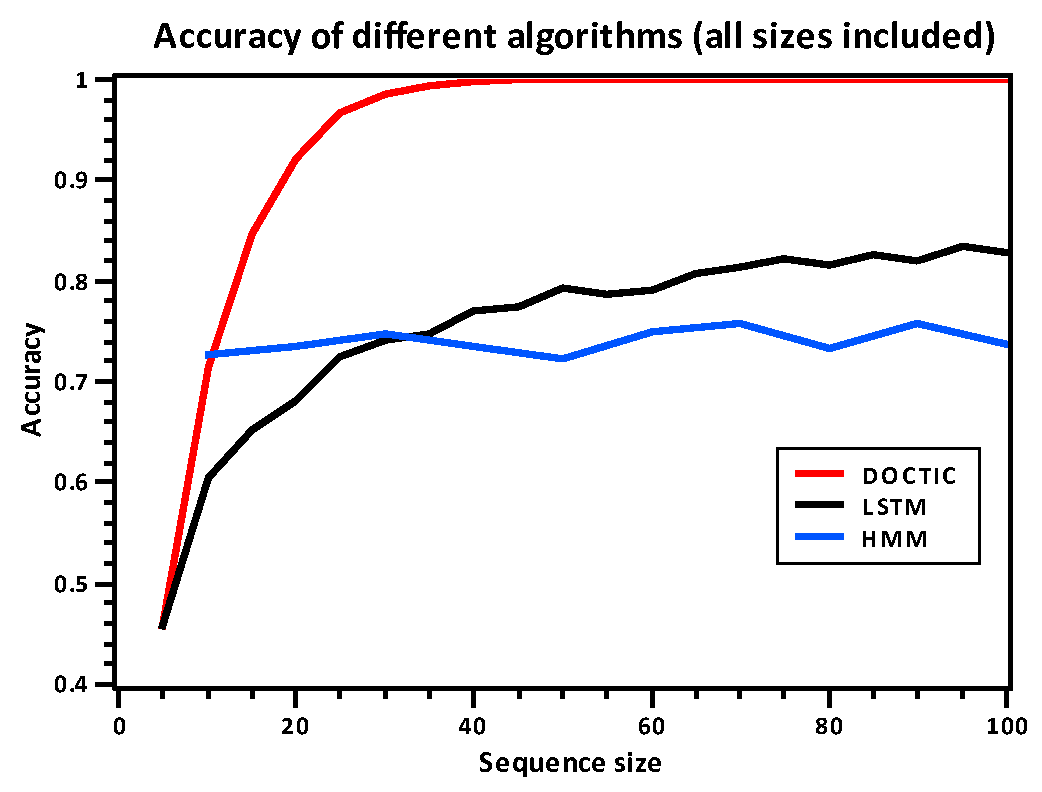
\includegraphics[width=\linewidth]{figs/accuracy_all.pdf}
		\caption{}
		\label{fig:timecost_cumulative}
	\end{subfigure}
	\begin{subfigure}{0.24\textwidth}
		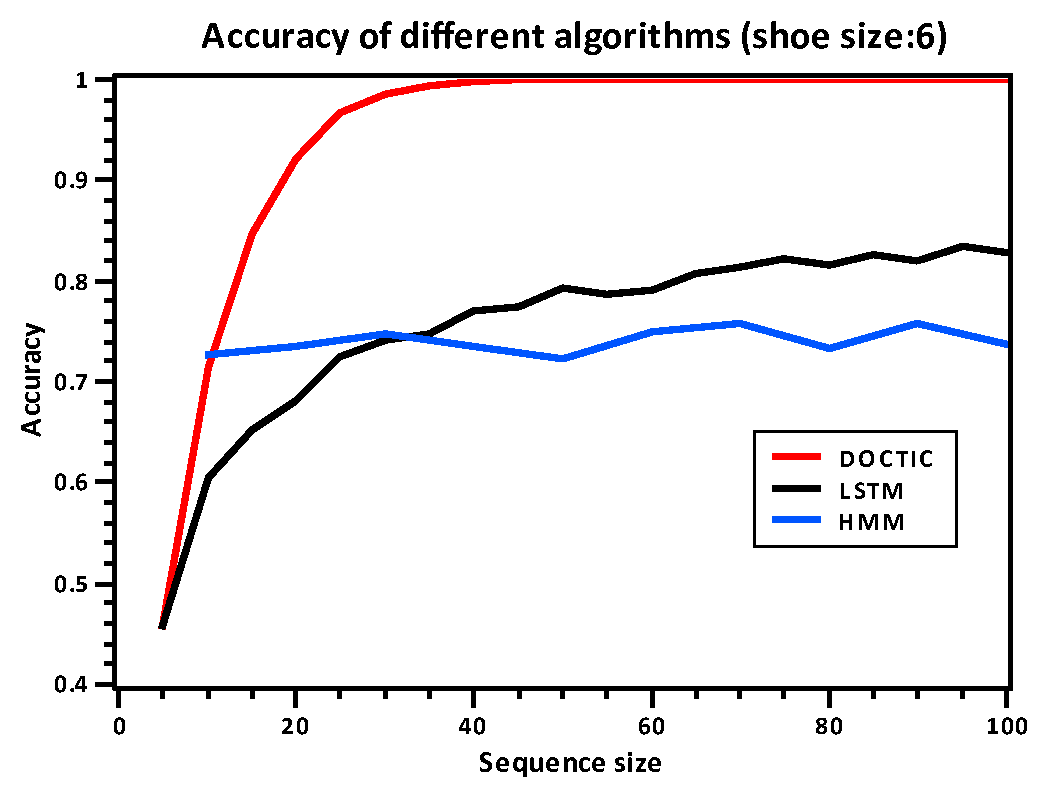
\includegraphics[width=\linewidth]{figs/accuracy_6.pdf}
		\caption{}
		\label{fig:accuracy_cumulative}
	\end{subfigure}
	\begin{subfigure}{0.24\textwidth}
		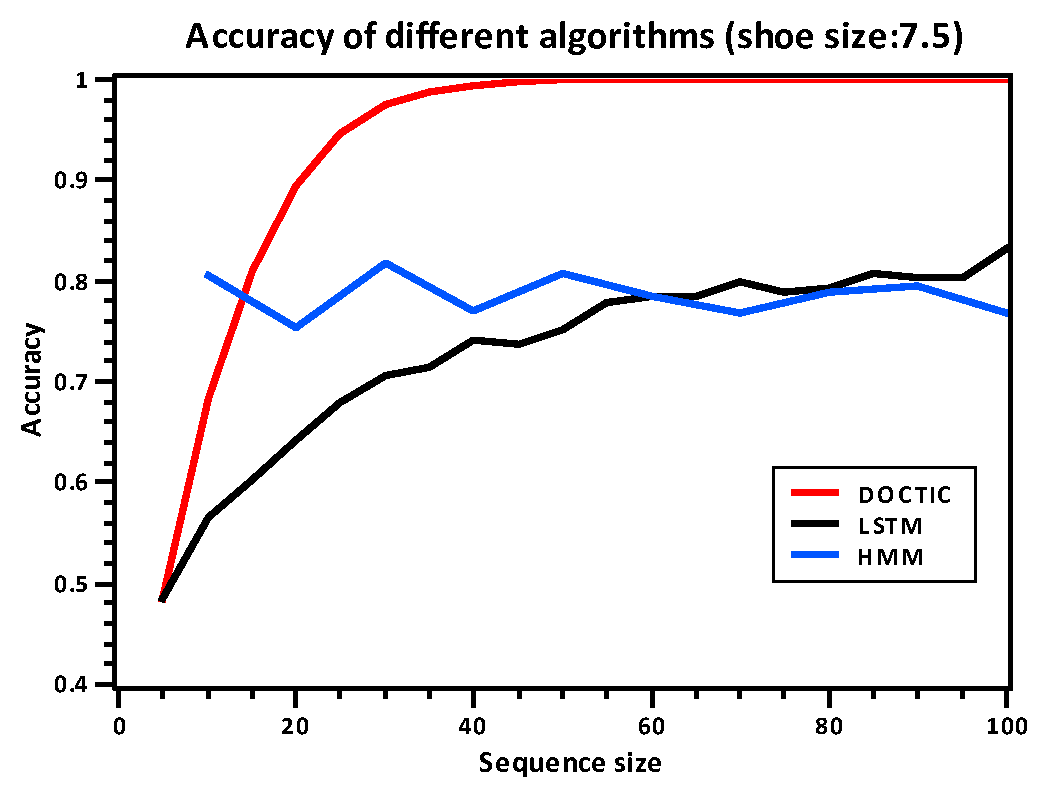
\includegraphics[width=\linewidth]{figs/accuracy_75.pdf}
		\caption{}
		\label{fig:timecost_cumulative}
	\end{subfigure}
	\begin{subfigure}{0.24\textwidth}
		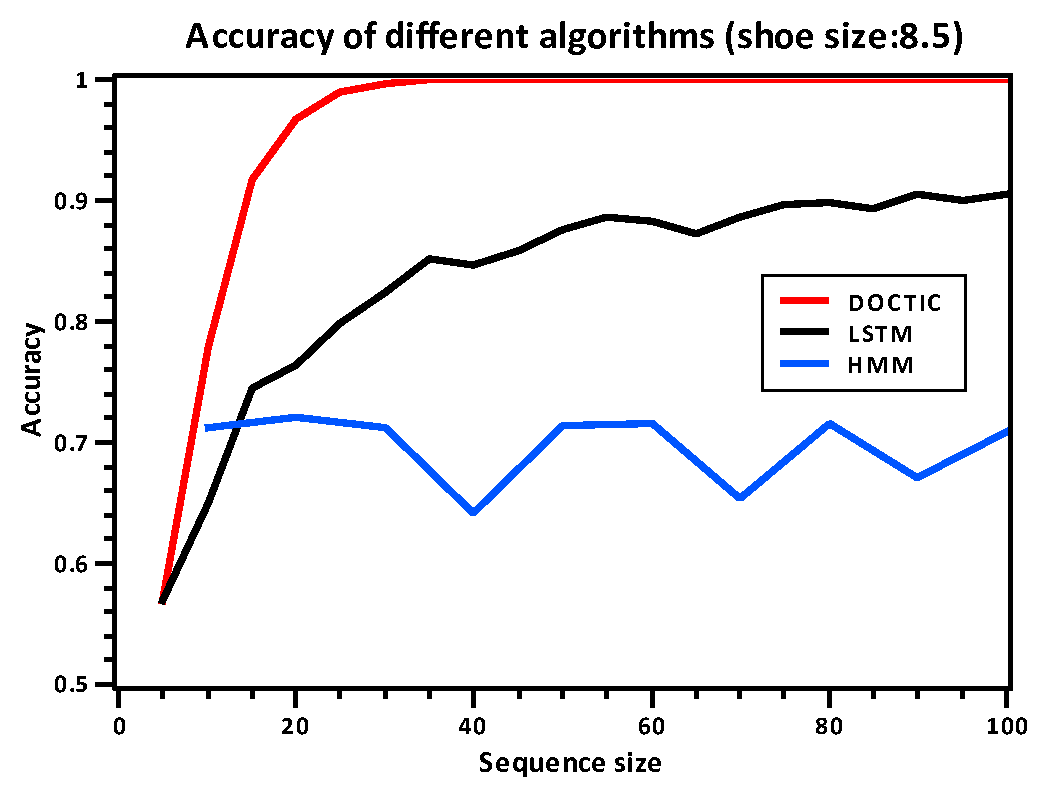
\includegraphics[width=\linewidth]{figs/accuracy_85.pdf}
		\caption{}
		\label{fig:accuracy_cumulative}
	\end{subfigure}	
	\caption{Accuracy comparison of \acs{hmm}, \acs{lstm} and \acs{doctic}, with different shoe sizes.}
	\label{fig:doctic}
\end{figure*}

%\subsection{Transition between different motion patterns}
%The classifier identifies the corresponding motion pattern for each sequence individually, however as an interactive application, it is critical to ensure that user experience is smooth and fast-responding.
%We analyze the transition latency between different motion patterns.
%Figure~\ref{fig:transition_matrix} presents the latency matrix for transitions between different motion patterns when the time length of the sequence sample is 1 second.
%The result shows that most transitions can be successfully detected within the range of [0.7, 0.8] seconds.

\section{Discussions}
\label{sec:discussions}
\subsection{Comparison with Existing WIP Method}
\label{sec:compare_wip}
%We here compare with the method of Low-Latency, Continuous-Motion for WIP \cite{feasel2008llcm}.
%This method computes the locomotion speed of virtual avatar based on the speed of the user's heel movement while walking in place.
%This existing work identifies two major challenges in WIP problems: system latency (particularly troublesome when starting and stopping movement), and the smooth and continuous change of user's viewpoint.

It is worth pointing out that the main purpose of this work differs from existing works in walking-in-place, including LLCM-WIP \cite{feasel2008llcm}, GUD-WIP \cite{wendt2010gud} and SAS-WIP \cite{bruno2013new}.
These existing methods are proposed to achieve walking-in-place with the amplitude, speed or frequency of foot movements.
They differ from our work in the focus of controlling the locomotion speed, or achieving the minimal latency between two states (start and stop). 
The goal of this work is to present a classification strategy which is capable of handling so-far the largest number of locomotion categories and adapting to pattern variations of different participants.

Concerning the latency performance, the metrics of starting and stopping latency of  LLCM-WIP \cite{feasel2008llcm} which specifically focuses on achieving low-latency interaction are 138 and 96 ms, less than 1/8 of a gait-cycle.
In comparison, our method requires more time (0.5 seconds) to detect the transition between 7 categories.
Despite the latency comparison, we improve the standard LLCM method in two ways: 1) avoid manual parameter adjustment, 2) address the pattern variations among different individuals.
The implementation of LLCM requires manual efforts of parameter adjustment, for example the cutoff frequency of the low-pass filter, as a tradeoff between smoothness of
locomotion and low latency.
The original work of LLCM focuses on the transition (start, stop) between two locomotion modes, and the challenge of parameter adjustment grows exponentially ($\mathbf{O}(N^2)$) with the number $N$ of locomotion categories.
The parameters are also expected to vary across different participants, increasing the complexity of parameter setting.
In contrast, our method avoids the manual settings of parameter values and inherently adapts to the variations across different individuals.


%The second challenge is related to the change of user's viewpoint.
%Current work sets the viewpoint based on the tracked orientation of the head-mounted VR device. 
%The forward direction is set to the same as the head orientation. 
%This consistency means that the user cannot adjust his/her viewpoints when moving in the virtual world. 
%This is proven not to be an important factor in the demonstrated experiments since the scenarios generally require the concentrated user attention when the participant is moving. 
%Users can freely adjust their viewpoint when standing still.

%However, computing the appropriate speed of virtual avatar is of great significance for better VR experience. Our current solution is to preset the speed based on multiple experiments which is difficult to meet the personalized walking style. It is undeniable that LLCM provides a considerable method, nevertheless, additional equipment to wear do cause the restricted action space and undesirable immersion experience. We expect to develop a decent method to solve this problem for future works. 



\subsection{Accuracy and Timecost Comparison with Existing Gesture Recognition Methods}
\label{sec:compare_performance}
Recognition algorithm is critical to correctly understand human activity.
So far, various methods have been proposed, including Dynamic Time Warping (DTW) \cite{mitsa2010temporal}, 
Markov Models \cite{bulling2008robust},  Conditional Random Fields \cite{blanke2010all} and Deep Neural Network (DNN) \cite{yang2015deep} etc.
Conventional methods such as DTW require feature selection by manually identifying contributing features during training and thereby reducing computational complexity during classification.
Readers may refer to a recent survey \cite{lara2013survey} for a tutorial on common techniques in feature extraction.


\paragraph{Comparison with HMM}Hidden Markov Model (HMM) has been widely used in the field of gesture recognition, achieving over 90\% success in KTH or Weizmann datasets in work \cite{sundaresan2003hidden}\cite{wilson1999parametric}\cite{chen2003hand}\cite{eickeler1998hidden}. Therefore, we compare with a HMM based approach to model actions using a modified Motion History Images (MHI) for feature extraction proposed by \cite{alp2017action}. They report 99\% success in Weizmann dataset. They modify the MHI by replacing the linear decay factor with an exponential decay factor emphasizing the recent motion more effectively so that HMM models can achieve a more recognition accuracy. In our implementation, MHI extracts the temporal features by obtaining the difference between the current moment and the previous moment and then computing the gradient direction. The HMM model is defined by $\lambda$= (A, B, $\pi$) with N number of states (in our problem, N=7). A is the transmission matrix, B comprises of the probability distributions for a feature vector extracted by MHI and $\pi$ is the initial distribution. $\lambda$ is trained for each motion categories separately using the observation sequence, the pressure signals from our insoles, with Baum and Welch algorithm. The Viterbi algorithm calculates the probability of each sequence in the test set to tell the final accuracy of this approach. After configuring HMM models with different parameters of hidden states (from 5 to 8) and training iteration (from 100 to 800), we evaluate the results and finally set the hidden states to be 7 and the training iteration to be 500. 

The time cost of one prediction is around 3 milliseconds. 
The results show that the full-size dataset achieves the accuracy around 75\% while the datasets with sizes of 6, 7.5, 8.5 achieve the level around 83\%, 79\%, 81\% respectively.
%indicating that HMM is sensitive to the sensor-specific variations as well as inter-person and intra-person variations. 
%Additionally, the size of the dataset is also a major factor affecting the performance considering that our data set (650 MB) is 2 times larger than Weizmann dataset (340 MB). 
%HMM is conspicuously dim in comparison with 
The results show that DOCTIC outperforms HMM in terms of accuracy and capability of coping with noisy and sparse sensor data.

\begin{table}[!htp]
	\def\arraystretch{1.25}
	\centering
	\begin{tabular}{C{1.5cm}C{2.3cm}C{1.5cm}C{2cm}}
		\hline
		& Ratio of Complete Dataset & Accuracy & Timecost per   sequence \\
		\hline\hline
		DTW        & 100\%                                                                 & 0.87     & 7585.13                                                           \\
		DTW        & 50\%                                                                  & 0.85     & 4021.45                                                              \\
		DTW        & 25\%                                                                  & 0.82     & 1936.34                                                              \\
		DTW        & 12.5\%                                                                  & 0.79     & 1013.11           \\  
		DTW        & 5.0\%                                                                  & 0.75     & 390.00                                                 \\
		DTW        & 1.0\%                                                                  & 0.57     & 77.55                                                 \\
		DTW        & 0.5\%                                                                  & 0.44    & 44.39                                                 \\
		LSTM & N/A                                                                   & 0.83     & 0.46          \\
		DOCTIC & N/A  & 0.97     & 13.64                                                \\\hline     
	\end{tabular}
	\caption{\label{tab:dtwlstm}Comparison of the accuracy and timecost for methods of DTW\&KNN and our method on the dataset of shoe size 8.5. Unit for the timecost is milliseconds and the sequence size is 100 for the standard \acs{lstm} and 25 for DOCTIC.}
\end{table}

\paragraph{Comparison with DTW $\&$ KNN}The combined recipe of Dynamic Time Warping (DTW) and  K Nearest Neighbors (KNN) is a representative method in the domain of time series classification \cite{mitsa2010temporal}.
This method is offline but is capable of achieving high accuracy given a large database.
We use this as a benchmark in terms of data size and accuracy.
The collected data is first processed by computing a vector of [mean, medium, max, min, standard deviation], given a segment of sensor data.
DTW aligns two vectors which are originally out of phase, then computes the corresponding distance between these aligned vectors. 
The label of the test sequence is predicted by finding the closest neighbor (K=1) in the training dataset. 
Research shows that this method achieves satisfactory accuracy for the task of time series classification \cite{xi2006fast}. 
However, this method is computationally too demanding for real-time applications, as in our case. 
One solution is to reduce the size of the dataset, which the incoming sequence is compared against. 
We use the technique of numerosity reduction \cite{xi2006fast, mitsa2010temporal} to reduce the dataset and accelerate the computation process. 
The results show that although the full-size dataset achieves the accuracy around 90\% (Table~\ref{tab:dtwlstm}), each attempt to find the closest neighbour in the dataset costs >7 seconds.
When reducing the dataset to speed up the computation, the accuracy drops significantly. 
Using larger number of features may potentially increase the accuracy but definitely lead to an explosion of the computing timecost.
In comparison, our method achieves an accuracy rate of 83\% at the cost of 0.46 milliseconds, in comparison to 82\% at the cost of 2 seconds for the method of DTW\&KNN when the dataset is maintained at 25\%.
This shows that the classifier built by our LSTM model captures the patterns embedded in the large dataset, thus can successfully detect the motion pattern without the need to individually compare against the samples in the complete database.
%The forward pass in the network is sufficiently fast to allow the classification in realtime.



\begin{figure}[!htp]
	\centering
	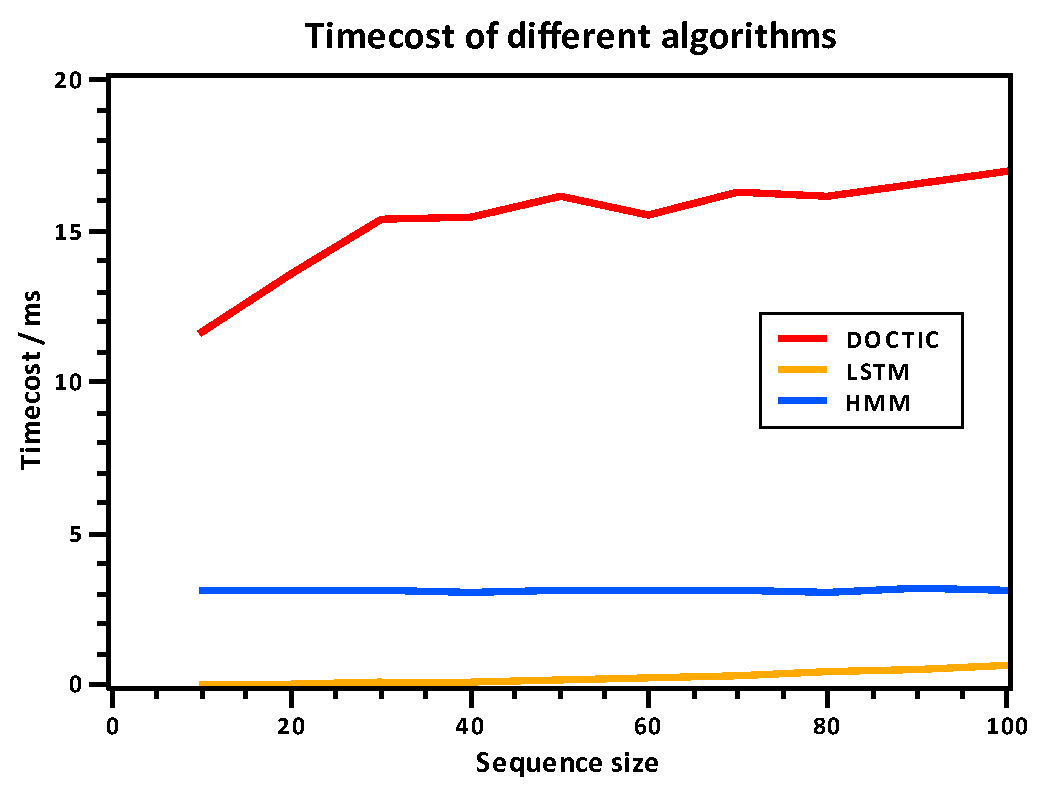
\includegraphics[width=\linewidth]{figs/timecost.pdf}
	\caption{Timecost comparison of \acs{hmm}, \acs{lstm} and \acs{doctic} with different sequence sizes.}
	\label{fig:timecost}
\end{figure}



\paragraph{Timecost Comparison}
Different sequence sizes critically affect the computation load and accuracy of the neural network.
For the standard LSTM method, the timecost increases from less than 0.1 to 0.6 millisecond when the sequence size increases from 10 (0.2 seconds) to 100 (2 seconds) (Figure~\ref{fig:timecost}).
The accuracy rate improves significantly from 50\% to over 80\% as the sequence size increases from 10 to 100 (Fig~\ref{fig:doctic}).
This indicates a longer sequence of data signal allows the classifier to better understand the embedded pattern and make the correct recognition.
However, it is worth noting that it requires the sample size to be over 75 (1.5 seconds) in order to reach an accuracy of 80\%.
Our proposed method, \acs{doctic}, improves the standard \acs{lstm} model by significantly shortening this time latency and increasing the accuracy rate.
Meanwhile, we found out that timecost of HMM is not significantly affected by the sequence size, though its accuracy improves when the sequence size increases.

With our iterative process in \acs{doctic}, the timecost increases 10 times as the standard \acs{lstm} model.
However, the maximal timecost is around 15 milliseconds (Figure~\ref{fig:timecost_cumulative}), still far less than the time gap between two data transmission (0.1 second).
Meanwhile the accuracy improves significantly for smaller segments of sequences.
A sequence size of 15 (0.3 seconds) can achieve an accuracy of 85.3\% (Figure~\ref{fig:accuracy_cumulative}), which is a comparable performance to the best accuracy from the standard \acs{lstm} model.
Furthermore, a sequence size of 25 improves the accuracy to 97.1\%.
This indicates that for most cases, the algorithm can produce the consensus of the predictions within a time window significantly smaller than the maximum sequence size (100).






%\subsection{Using Different Sequence Sizes for the Improved Method with \acs{doctic}}





\section{Applications}
\label{sec:applications}
Given the characteristics of high accuracy and low latency of our DOCTIC classification method, this interaction technique with smart insoles  has great potential to be applied to a wide range of real-time VR applications.
% yielding a more intuitive and immersive interaction experience for VR as opposed to conventional joystick or handle based control mode. 



On one hand, the high accuracy guarantees the stable prediction of foot gesture, which is significant for applications involving consistent and continuous gestures. We reconstruct a virtual lab environment with the same layout as our real one with room size 12$\times$9.6 square meters. Participants wearing the VR device are asked to navigate through the lab in the mode of real walking (Figure~\ref{fig:lab}). We record the movement of the participant and his/her perspective in the virtual environment. In this scenario, the forward walking is achieved with real walking. 
Besides the continuous and accurate prediction of walking pattern, the virtual velocity also assumes a significant role in preventing users from colliding with objects in real world. 
In our current implementation, the velocity of the virtual character is set to 0.384 m/s. 
The actual moving velocity of the participant is 0.8 m/s. 
The misperception between the virtual and real walking speed has been investigated by a recent work \cite{nilsson2016perceived}, and it could be one of our future works to investigate which factors may cause such misperception in our scenario.
\begin{figure}[!htpb]
	\centering
	\begin{subfigure}{0.44\linewidth}
		\centering
		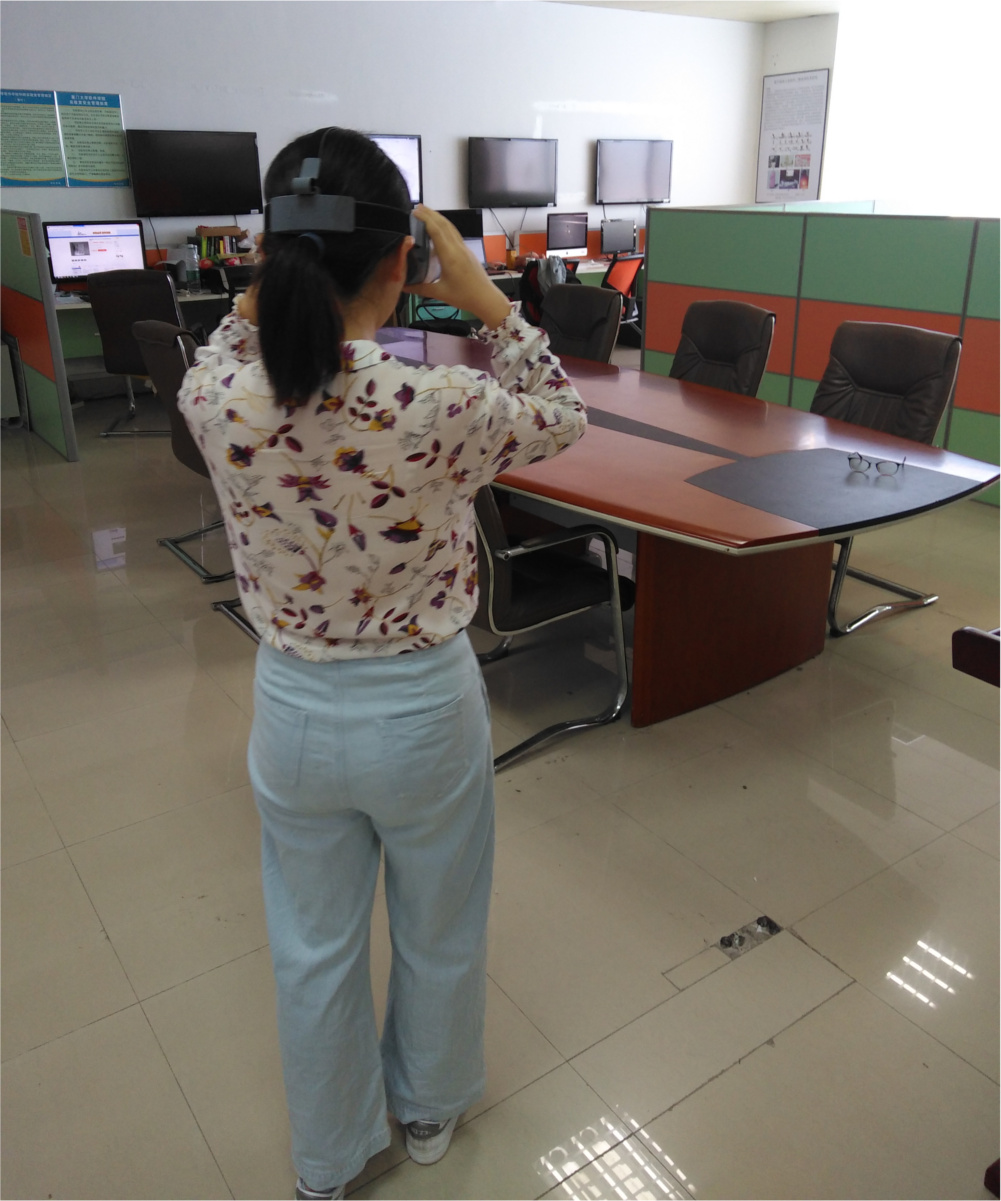
\includegraphics[width=\linewidth]{./figs/lab_real.jpg}
		\caption[]{\label{fig:lab_real} Participant In Action
		}
	\end{subfigure}
	~
	\begin{subfigure}{0.44\linewidth}
		\centering	
		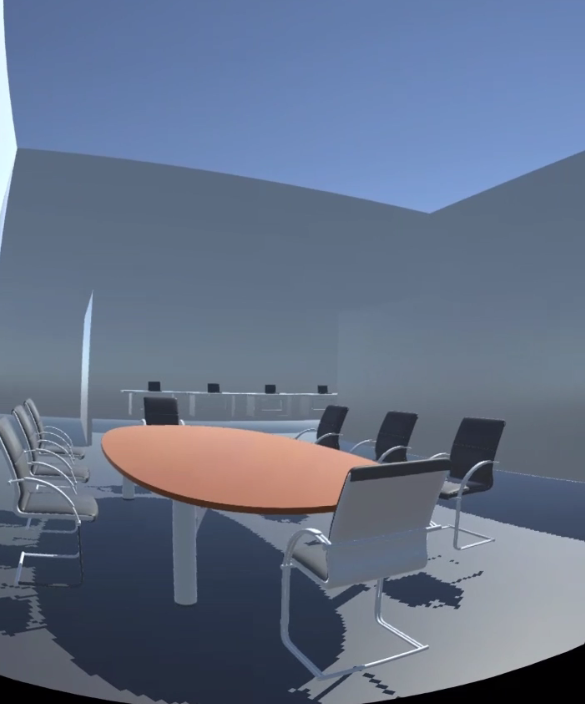
\includegraphics[width=\linewidth]{./figs/lab_virtual.png}
		\caption[]{\label{fig:lab_virtual} First-person View
		}
	\end{subfigure}	
	~
	\\
	\begin{subfigure}{\linewidth}
		\centering	
		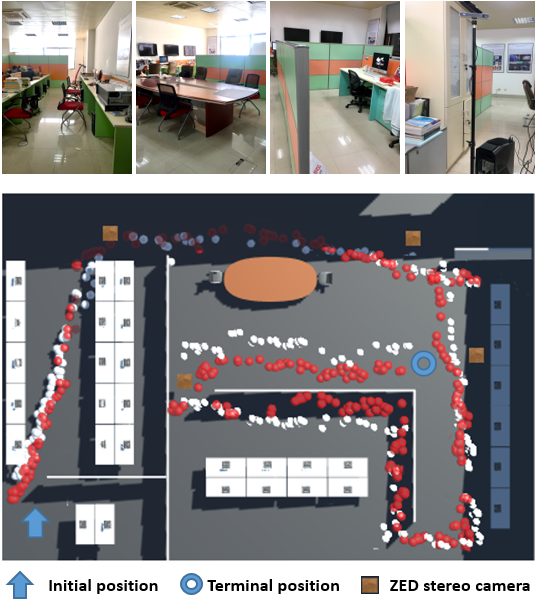
\includegraphics[width=0.90\linewidth]{./figs/lab_comparison.png}
		\caption[]{\label{fig:lab_comparison} Trajectory Comparison
		}
	\end{subfigure}				
	\caption[]{\label{fig:lab}
		Interactive demo of real walking in a virtual lab.
	}
\end{figure}

We tracked the trajectory of the participant in RW with 4 stereo cameras (ZED) placed in different locations in the lab.
2D body postures are tracked with the open-source project, OpenPose \cite{cao2017realtime}, and 3D posture is reconstructed with the calibration information of stereo images.
The detected body center (hip) is selected as the world coordinate of the participant in RW.
The average time cost to complete the travelling distance of 45 meters is around 55 seconds. 
Figure~\ref{fig:lab_comparison} shows that the trajectory in RW (marked in white dots) and the trajectory in VE (marked in red dots) are roughly similar, the average Euclidean distance between the two is 6.38cm, indicating the robust recognition performance for a relatively long distance.


On the other hand, it has the capacity, rooted in the low latency, to satisfy the smooth requirement of real-time VR games with frequent switching of multiple movements. This can be demonstrated with an example of a first-person shooting game, named as \emph{Zombie Town} (Figure~\ref{fig:zombie}), receiving praise from volunteers. The size of the virtual space is 72$\times$72 square meters, with a total number of 17 zombies. 
The \emph{referent} action of walking forward is triggered with the technique of walking-in-place.
Users navigate inside this environment with the foot gestures and shoot the avatars with the handle. 
Users aim at shooting the zombies while traversing the challenging environment (such as stacked obstacles).
Various gestures, standing/walking/running/jumping, are needed in order to accomplish the task. 
\begin{figure}[h]
	\centering
	\begin{subfigure}{0.47\linewidth}
		\centering
		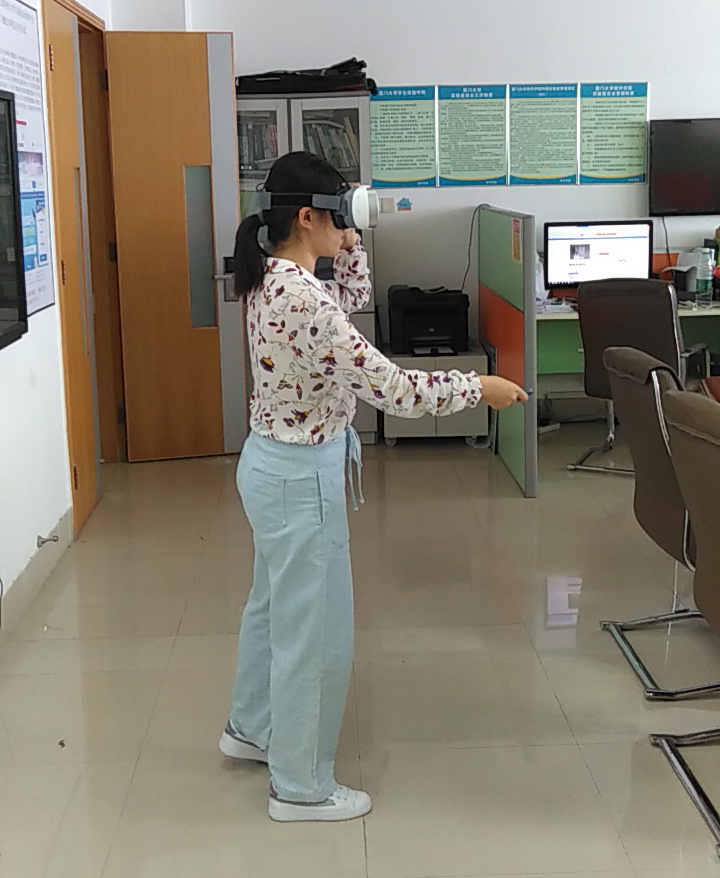
\includegraphics[width=\linewidth]{./figs/zombie_real.jpg}
		\caption[]{\label{fig:zombie_real} Participant In Action
		}
	\end{subfigure}
	~
	\begin{subfigure}{0.47\linewidth}
		\centering	
		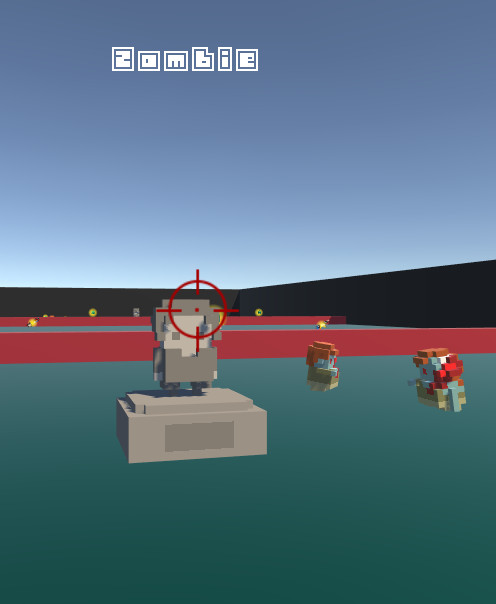
\includegraphics[width=\linewidth]{./figs/zombie_virtual.jpg}
		\caption[]{\label{fig:zombie_virtual} First-person View
		}
	\end{subfigure}		
	\caption[]{\label{fig:zombie}
		Interactive demo of Zombie Town.
	}
\end{figure}
%In this case, we compare the proposed method of using smart insoles with the use of handle as a baseline. 
%We compare the number of zombies being shot using these two different interaction techniques within a fixed time window of 1 minute. 
%We ensure that the experience time of each participant is no less than 5 minutes.


% Our implementations of VR application instance are conspicuously pretty simple, however, there are great chance for far more elaborate designed VR applications not limited to the scenes and areas we mentioned. 

% We reconstruct a virtual lab environment with the same layout as our real one with room size 12$\times$9.6 meters.
% Participants wearing the VR device are asked to navigate through the lab in the mode of real walking (Figure~\ref{fig:lab}).
% We record the movement of the participant and his/her perspective in the virtual environment.
% In this scenario, the forward walking is achieved with real walking.

% We tracked the trajectory of the participant in RW with 4 stereo cameras (ZED) placed in different locations in the lab.
% 2D body postures are tracked with the open-source project, OpenPose \cite{cao2017realtime}, and 3D posture is reconstructed with the calibration information of stereo images.
% The detected body center (hip) is selected as the world coordinate of the participant in RW.
% Figure~\ref{fig:lab_comparison} shows that the trajectory in RW (marked in white dots) and the trajectory in VE (marked in red dots) are roughly similar indicating the robust recognition performance for a relatively long distance.
% Besides the continuous and accurate prediction of walking pattern, the virtual velocity also assumes a significant role in preventing users from colliding with objects in real world.
% In our current implementation, the velocity of the virtual character is set to 0.384 m/s.
% The actual moving velocity of the participant is 0.8 m/s.

% The average time cost to complete the travelling distance of 45 meters is around 55 seconds. 

% \subsection{Virtual Track}
% A virtual track is set up to verify the accuracy of DOCTIC for each individual motion in real-world scenarios, with separate segments indicating users to perform the corresponding patterns (Figure~\ref{fig:track}).
% The track size is 86.4$\times$52.8 meters.
% In particular, a series of hurdles are arranged (at the bottom side on Figure~\ref{fig:track_layout}) so that the participant needs to jump over the hurdles consecutively.
% The participant is placed at the beginning of the segment \emph{walking forward} (marked as red dot in Figure~\ref{fig:track_layout}), and terminates at the same position.
% For the segment of \emph{walking backward}, the viewpoint is rotated 180 degrees so the virtual character walks backward and returns to the starting point.
% The room in RW is sufficiently large to allow the participant to walk backwards with no safety concern of object collision.
% In this scenario, the forward walking is achieved with walking-in-place.

% In this case, we collected the mis-labelled actions for each segment.
% The accuracy is 85\% for the segments of walking forward, running, jumping, walking left, walking right, and walking backward. 

% The average time cost to complete the task is around 60 seconds.

% \begin{figure}[!htpb]
% 	\centering
% 	\begin{subfigure}{0.40\linewidth}
% 		\centering
% 		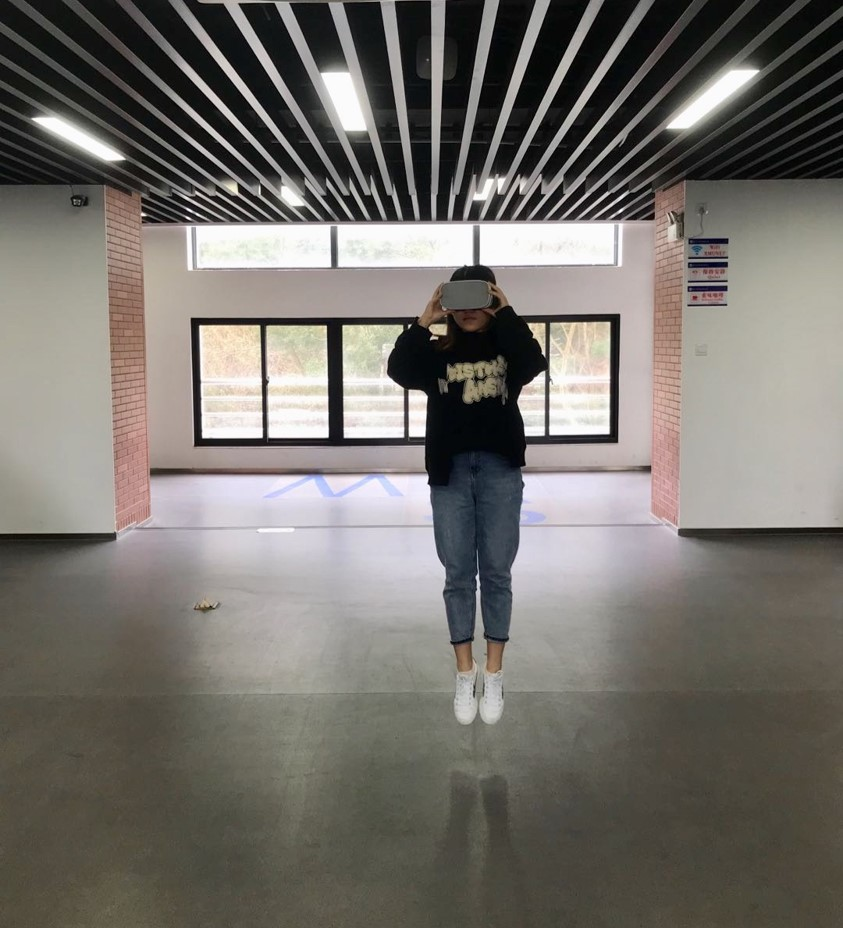
\includegraphics[width=\linewidth]{./figs/track_real.png}
% 		\caption[]{\label{fig:track_real} Participant In Action
% 		}
% 	\end{subfigure}
% 	~
% 	\begin{subfigure}{0.40\linewidth}
% 		\centering
% 		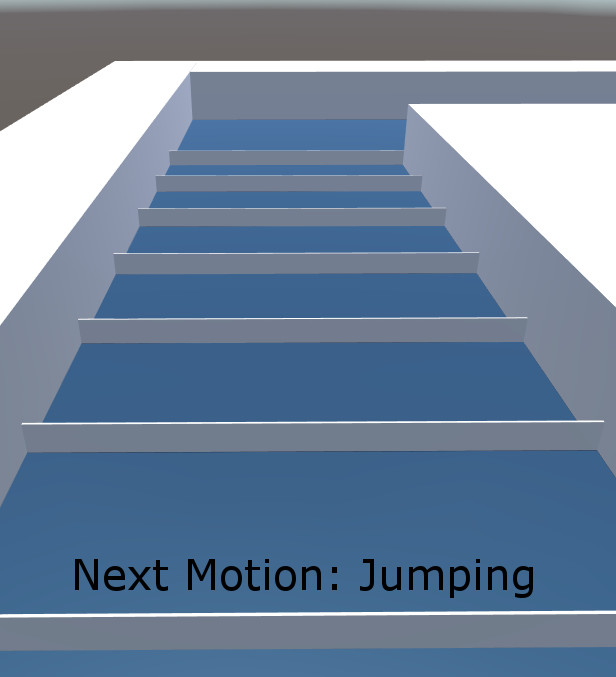
\includegraphics[width=\linewidth]{./figs/track_close.jpg}
% 		\caption[]{\label{fig:track_close} Jumping Section
% 		}
% 	\end{subfigure}
% 	~
% 	\\
% 	\begin{subfigure}{0.8\linewidth}
% 		\centering	
% 		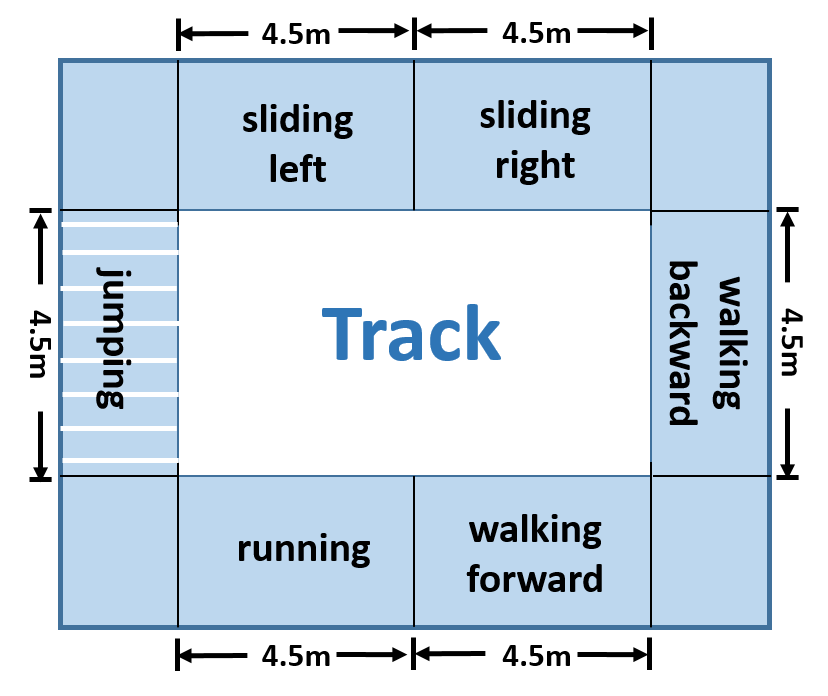
\includegraphics[width=\linewidth]{./figs/track_layout.png}
% 		\caption[]{\label{fig:track_layout} Top View
% 		}
% 	\end{subfigure}			
% 	\caption[]{\label{fig:track}
% 		Interactive demo of navigating in a virtual track.
% 	}
% \end{figure}

% \subsection{Zombie Town}
% A first-person shooting game, named as \emph{Zombie Town} (Figure~\ref{fig:zombie}), is developed.
% Users navigate inside this environment with the foot gestures and shoot the avatars with the handle. 
% Users need to use various gestures, standing/walking/running/jumping, in order to traverse challenging environment (such as stacked obstacles).
% The size of the virtual space is  72$\times$72 meters, with a total number of 17 zombies.
% In this scenario, the forward walking is achieved with walking-in-place.

% In this case, we compare the proposed method of using smart insoles with the use of handle as a baseline.
% We compare the number of zombies being shot using these two different interaction techniques within a fixed time window of 1 minute.
% We ensure that the experience time of each participant is no less than 5 minutes.

% % it is hard to beat the handle, but user experiences are better since it involves their real body actions.



% \subsection{Qualitative Evaluation with Questionnaire}
% After completing all three aforementioned experiments, participants are asked to rate the naturalness, latency and accuracy of this interaction mode (Table~\ref{tab:finalQ}).
% Questions of Q1 - Q3 receive an average scores of 3.9, 3.2, 3.5, with standard deviations of 0.74, 0.63, 0.71 respectively.
% The score distribution is presented in Figure~\ref{fig:final_scores}. 
% The results show that most users are satisfied with the performance in three aspects.
% In particular, participants rated the aspect of naturalness with higher score.

% Participants are invited to conduct the experiments with the control of conventional joystick.
% The comparison between the joystick and our proposed method is supported by the responses of Q4, where 8 out of 10 participants choose our proposed method over the standard joystick.
% Participants are surprised by the high consistency of walking in both virtual and real lab, and also attracted by the application of Zombie Town.
% Some comments from the participants are: "I cannot feel the latency for most of the time", "The recognition accuracy is excellent."
% For the jumping section in the demo of virtual track, one participant suggested including the action of jumping on one foot, in addition to the current action of jumping on both feet.

% We did not explicitly ask participants to fill in Questionnaire~\ref{tab:finalQ}, but collected subjective comments from participants after each experiment.
% The use of foot gestures in the experiments of virtual lab and zombie town receives more positive feedback from users than the experiment of virtual track.
% Since participants completed the experiments at a random order, the feedback is not affected by the sequential order of the experiments.
% For the case of virtual lab, it could be caused by the mode of real-walking, offering higher immersion in comparison to walking-in-place.
% For the case of zombie town, the intense game-like scenario increases participants' involvement and concentration, leading to a higher rating of our interaction mode.
% While users are asked to repeat the same action for a certain period in the experiment of virtual track, the experience of repetition could be the reason for the down-graded popularity.
% This also informs that the use of foot gestures can be more potentially useful for relevant scenarios.



% \begin{table}[!htp]
% 	\def\arraystretch{1.25}
% 	\centering
% 	\begin{tabular}{C{1cm}p{7cm}}
% 		\hline
% 		Score & Description of Criteria       \\
% 		\hline \hline
% 		Q1 & Please rate the naturalness of the interaction from 1 (unnatural) to 5 (natural) \\
% 		Q2 & Please rate the experience of recognition latency from 1 (high latency) to 5 (low latency)\\		
% 		Q3 & Please rate the recognition accuracy from 1 (low) to 5 (high) \\   
% 		Q4 & Will you choose the smart insoles instead of the joystick?\\
% 		\hline               
% 	\end{tabular}
% 	\caption{\label{tab:finalQ} Questionnaire after participants experience the validation demos. }
% 	% For detailed description, please refer to supplementary document.}
% \end{table}




%\begin{table}[!htp]
%	\def\arraystretch{1.25}
%	\centering
%	\begin{tabular}{C{1cm}p{7cm}}
%		\hline
%		Score & Description of Criteria       \\
%		\hline \hline
%		1 & Extremely different from natural movements and completely unnatural \\
%		2 & Largely different from natural movements and require intensive attention to perform the actions \\
%		3 & Slightly different from natural motions but acceptable interaction\\   
%		4 & Similar to natural motions and provide good experience\\
%		5 & High consistency with natural motions and provide immersive experience\\
%		\hline               
%	\end{tabular}
%	\caption{\label{tab:Q3} Q3 Please rate the naturalness of using these foot patterns for interaction. }
%	% For detailed description, please refer to supplementary document.}
%\end{table}
%
%
%\begin{table}[!htp]
%	\def\arraystretch{1.25}
%	\centering
%	\begin{tabular}{C{1cm}p{7cm}}
%		\hline
%		Score & Description of Criteria       \\
%		\hline \hline
%		1 & Significant delay and unable to properly engage in the applications \\
%		2 & Large delay and disturbing experience \\
%		3 & Moderate but acceptable delay, does not affect the interaction \\   
%		4 & Cannot feel the delay for most of the time, but experience some delay between motion transition\\
%		5 & Almost feel no delay\\
%		\hline               
%	\end{tabular}
%	\caption{\label{tab:Q1} Q1 Please rate the recognition latency in these demos. }
%	% For detailed description, please refer to supplementary document.}
%\end{table}
%
%\begin{table}[!htp]
%	\def\arraystretch{1.25}
%	\centering
%	\begin{tabular}{C{1cm}p{7cm}}
%		\hline
%		Score & Description of Criteria       \\
%		\hline \hline
%		1 & Completely wrong, almost none of my motions are recognized correctly  \\
%		2 & Only a few attempts are recognized correctly \\
%		3 & The majority of the attempts are recognized correct\\   
%		4 & Satisfactory accuracy, though a few attempts are wrong\\
%		5 & Significantly high accuracy\\
%		\hline               
%	\end{tabular}
%	\caption{\label{tab:Q2} Q2 Please rate the recognition accuracy in these demos. }
%	% For detailed description, please refer to supplementary document.}
%\end{table}


% \section{Discussions}

% %\subsection{Comparing the Classification Performance on Individual Shoe Sizes}


% \subsection{Normalization of Individual Variation}
% The only post-processing procedure when preparing the training dataset is to normalize the data with the maximal sensor-specific value for individual participants.
% However, when running the application in real-time, it is challenging to estimate such 'maximal' values within a short time interval.
% The current solution is to set up a starting stage when users are guided to perform a few actions before starting the main application.
% The algorithm estimates these 'maximal' values based on the collected data during this stage.
% These parameters are dynamically updated as a user is engaging in this application.
% How to fast estimate such parameters is critical to maintain a high accuracy at the initial stage of the application.

\section{Conclusion}
\label{sec:conclusion}
Our work uses foot patterns as the interaction mode for locomotion in a virtual environment. 
The proposed method, DOCTIC, can accurately classify user activities into seven categories: standing, walking forward/backward, running, jumping, sliding left/right. 
The main contribution of this work is the capability of accurate and fast classification of foot patterns with noisy and sparse inputs. 
We conducted experiments and showed that using foot patterns can provide intuitive interaction for VR applications. 

For future works, we are developing an intelligent classifier which adapts to a specific user and insoles.
Using the current classifier as an initial template, we plan to continuously collect the data flow of the specific user and insoles, and incrementally improve the accuracy of classification.
This strategy is promising in completely removing the variations in inter-person patterns and sensor specifics.
We expect to achieve a considerably high accuracy of pattern recognition and plan to extend the pattern repertoire to include daily and athletic movements.
Another future direction is posture reconstruction based on the information of plantar pressure. 
We hypothesize that the body posture, in particular the lower-body posture, critically determines the pressure distribution on the feet, which could be used to reversely infer the current posture. 
This can be used to track the body movement when the user is wearing the smart insole, and be used in applications including rehabilitation, interaction games etc.
However, the technical challenge lies in constructing the mapping from the limited, noisy and sparse pressure information to the high-dimensional body configuration. 



% \begin{table}
%   \caption{Frequency of Special Characters}
%   \label{tab:freq}
%   \begin{tabular}{ccl}
%     \toprule
%     Non-English or Math&Frequency&Comments\\
%     \midrule
%     \O & 1 in 1,000& For Swedish names\\
%     $\pi$ & 1 in 5& Common in math\\
%     \$ & 4 in 5 & Used in business\\
%     $\Psi^2_1$ & 1 in 40,000& Unexplained usage\\
%   \bottomrule
% \end{tabular}
% \end{table}

% \begin{acks}
%   The authors would like to thank Dr. Yuhua Li for providing the
%   MATLAB code of the \textit{BEPS} method.

%   The authors would also like to thank the anonymous referees for
%   their valuable comments and helpful suggestions. The work is
%   supported by the \grantsponsor{GS501100001809}{National Natural
%     Science Foundation of
%     China}{http://dx.doi.org/10.13039/501100001809} under Grant
%   No.:~\grantnum{GS501100001809}{61273304}
%   and~\grantnum[http://www.nnsf.cn/youngscientists]{GS501100001809}{Young
%     Scientists' Support Program}.

% \end{acks}
%% if specified like this the section will be committed in review mode
\acknowledgments{
This work is supported by National Natural Science Foundation of China (61702433, 61661146002).}

%\bibliographystyle{abbrv}
\bibliographystyle{abbrv-doi}
%\bibliographystyle{abbrv-doi-narrow}
%\bibliographystyle{abbrv-doi-hyperref}
%\bibliographystyle{abbrv-doi-hyperref-narrow}

\bibliography{acmart}
\end{document}
